\section{Continuous random variables}

\mode<presentation>{
%---------------------------------------------------------------------slide----
\begin{frame}
\frametitle{Continuous random variables}

\tableofcontents[sectionstyle=show/hide,hideothersubsections]
\end{frame}
}


\subsection{Variables aleatorias continuas}

%---------------------------------------------------------------------slide----
\begin{frame}
\frametitle{Continuous random variables}
Continuous random variables, unlike discrete random variables, can take any value in a real interval. 
Thus the range of a continuous random variables is infinite and uncountable. 

Such a density of values makes impossible to compute the probability for each one of them, and therefore, it's not
possible to define a probabilistic model trough a probability function like with discrete random variables.

Besides, usually the measurement of continuous random variable is limited by the precision of the measuring instrument.
For instance, when somebody says that is $1.68$ meters tall, his or her true height is no exactly $1.68$ meters, cause
the precision of the measuring instrument is only cm (two decimal places). 
This means that the true height of that person is between $1.675$ y $1.685$ meters.

Hence, for continuous variables, \alert{\emph{it make no sense to calculate the probability of an isolated value, and we
will calculate probabilities for intervals.}}
\end{frame}


%---------------------------------------------------------------------slide----
\begin{frame}
\frametitle{Probability density function}
To model the probability distribution of a continuous random variable is used a probability density function.

\begin{definition}[Probability density function]
The \emph{probability density function} of a continuous random variable $X$ is a function $f(x)$ that meets the
following conditions:
\begin {itemize}
\item Is non-negative: $f(x)\geq 0$ $\forall x\in \mathbb{R}$,
\item The area bounded by the curve of the density function and the x-axis is equal to 1, that is,
\[
\int_{-\infty}^{\infty} f(x)\; dx = 1.
\]
\item The probability that $X$ assumes a value between $a$ and $b$ is equal to the area under the density function
bounded by $a$ and $b$, that is,
\[
P(a\leq X\leq b) = \int_a^b f(x)\; dx
\]
\end{itemize}
\end{definition}

The probability density function measures the relative likelihood of every value, but \alert{\emph{Watch out!, $f(x)$ is
not the probability of $x$.}}, cause $P(X=x)=0$ for every $x$ value by definition.
\end{frame}


%---------------------------------------------------------------------slide----
\begin{frame}
\frametitle{Distribution function}
The same way that for discrete random variables, for continuous random variables it makes sense to calculate cumulative
probabilities.
\begin{definition}[Distribution function]
The \emph{distribution function} of a continuous random variable $X$ is a function $F(x)$ that maps every value $a$ to
the probability that $X$ takes on a value less than or equal to $a$, that is,
\[
F(a) = P(X\leq a) = \int_{-\infty}^{a} f(x)\; dx.
\]
\end{definition}

\end{frame}


%---------------------------------------------------------------------slide----
\begin{frame}
\frametitle{Probabilities as areas}

\begin{center}
\tikzsetnextfilename{continuous_random_variables/density_function}
\mode<article>{\resizebox{0.7\textwidth}{!}{% Created by tikzDevice version 0.9 on 2016-04-28 16:54:50
% !TEX encoding = UTF-8 Unicode
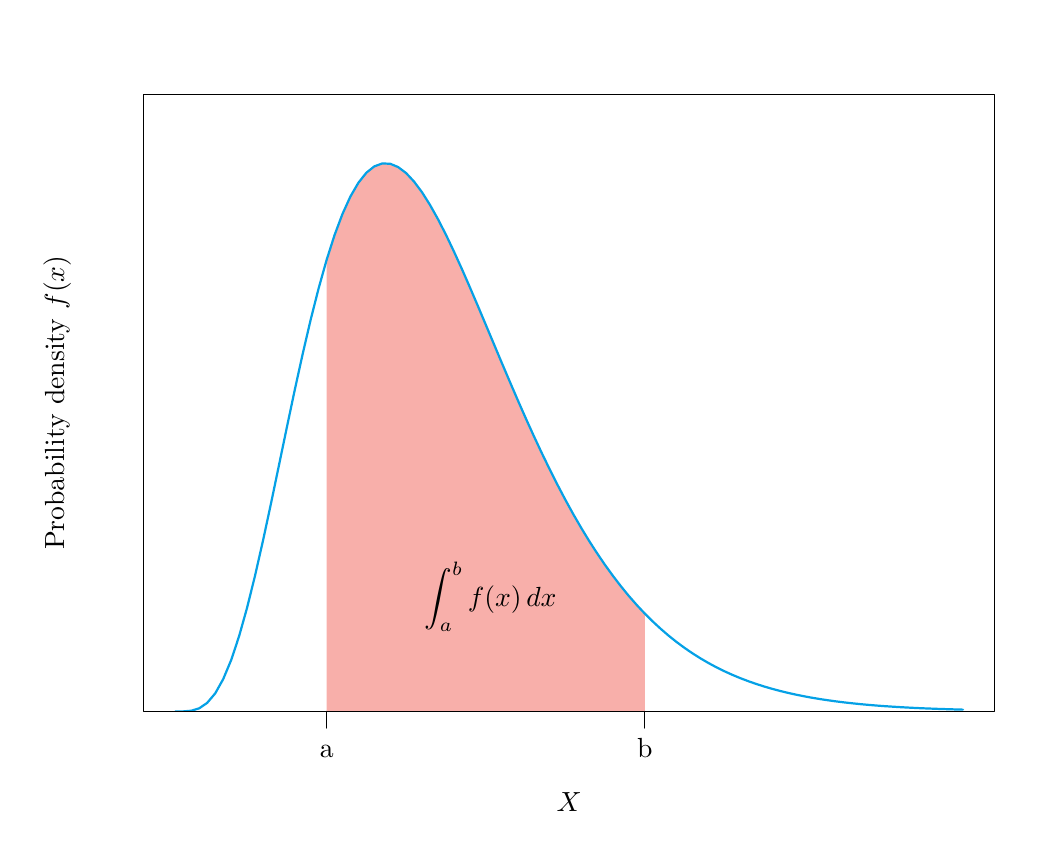
\begin{tikzpicture}[x=1pt,y=1pt]
\definecolor{fillColor}{RGB}{255,255,255}
\path[use as bounding box,fill=fillColor,fill opacity=0.00] (0,0) rectangle (361.35,289.08);
\begin{scope}
\path[clip] (  0.00,  0.00) rectangle (361.35,289.08);
\definecolor{drawColor}{RGB}{0,0,0}

\node[text=drawColor,anchor=base,inner sep=0pt, outer sep=0pt, scale=  1.00] at (195.67,  6.00) {$X$};

\node[text=drawColor,rotate= 90.00,anchor=base,inner sep=0pt, outer sep=0pt, scale=  1.00] at ( 13.20,153.54) {Probability density $f(x)$};
\end{scope}
\begin{scope}
\path[clip] (  0.00,  0.00) rectangle (361.35,289.08);
\definecolor{drawColor}{RGB}{0,0,0}

\path[draw=drawColor,line width= 0.4pt,line join=round,line cap=round] (108.00, 42.00) -- (222.98, 42.00);

\path[draw=drawColor,line width= 0.4pt,line join=round,line cap=round] (108.00, 42.00) -- (108.00, 36.00);

\path[draw=drawColor,line width= 0.4pt,line join=round,line cap=round] (222.98, 42.00) -- (222.98, 36.00);

\node[text=drawColor,anchor=base,inner sep=0pt, outer sep=0pt, scale=  1.00] at (108.00, 25.20) {a};

\node[text=drawColor,anchor=base,inner sep=0pt, outer sep=0pt, scale=  1.00] at (222.98, 25.20) {b};
\end{scope}
\begin{scope}
\path[clip] ( 42.00, 42.00) rectangle (349.35,265.08);
\definecolor{fillColor}{RGB}{238,50,36}

\path[fill=fillColor,fill opacity=0.39] (108.00, 42.00) --
	(108.00,205.09) --
	(110.87,214.08) --
	(113.75,221.76) --
	(116.62,228.08) --
	(119.50,233.03) --
	(122.37,236.65) --
	(125.25,238.95) --
	(128.12,240.01) --
	(131.00,239.90) --
	(133.87,238.71) --
	(136.75,236.53) --
	(139.62,233.46) --
	(142.50,229.60) --
	(145.37,225.05) --
	(148.24,219.92) --
	(151.12,214.30) --
	(153.99,208.28) --
	(156.87,201.95) --
	(159.74,195.38) --
	(162.62,188.66) --
	(165.49,181.84) --
	(168.37,174.99) --
	(171.24,168.15) --
	(174.12,161.39) --
	(176.99,154.73) --
	(179.86,148.21) --
	(182.74,141.86) --
	(185.61,135.71) --
	(188.49,129.77) --
	(191.36,124.06) --
	(194.24,118.58) --
	(197.11,113.35) --
	(199.99,108.38) --
	(202.86,103.65) --
	(205.74, 99.18) --
	(208.61, 94.96) --
	(211.49, 90.98) --
	(214.36, 87.24) --
	(217.23, 83.73) --
	(220.11, 80.44) --
	(222.98, 77.38) --
	(222.98, 42.00) --
	cycle;
\definecolor{drawColor}{RGB}{5,161,230}

\path[draw=drawColor,line width= 0.8pt,line join=round,line cap=round] ( 53.38, 42.00) --
	( 56.26, 42.02) --
	( 59.13, 42.26) --
	( 62.01, 43.14) --
	( 64.88, 45.11) --
	( 67.76, 48.52) --
	( 70.63, 53.63) --
	( 73.51, 60.51) --
	( 76.38, 69.14) --
	( 79.25, 79.36) --
	( 82.13, 90.94) --
	( 85.00,103.57) --
	( 87.88,116.95) --
	( 90.75,130.71) --
	( 93.63,144.55) --
	( 96.50,158.14) --
	( 99.38,171.21) --
	(102.25,183.52) --
	(105.13,194.86) --
	(108.00,205.09) --
	(110.87,214.08) --
	(113.75,221.76) --
	(116.62,228.08) --
	(119.50,233.03) --
	(122.37,236.65) --
	(125.25,238.95) --
	(128.12,240.01) --
	(131.00,239.90) --
	(133.87,238.71) --
	(136.75,236.53) --
	(139.62,233.46) --
	(142.50,229.60) --
	(145.37,225.05) --
	(148.24,219.92) --
	(151.12,214.30) --
	(153.99,208.28) --
	(156.87,201.95) --
	(159.74,195.38) --
	(162.62,188.66) --
	(165.49,181.84) --
	(168.37,174.99) --
	(171.24,168.15) --
	(174.12,161.39) --
	(176.99,154.73) --
	(179.86,148.21) --
	(182.74,141.86) --
	(185.61,135.71) --
	(188.49,129.77) --
	(191.36,124.06) --
	(194.24,118.58) --
	(197.11,113.35) --
	(199.99,108.38) --
	(202.86,103.65) --
	(205.74, 99.18) --
	(208.61, 94.96) --
	(211.49, 90.98) --
	(214.36, 87.24) --
	(217.23, 83.73) --
	(220.11, 80.44) --
	(222.98, 77.38) --
	(225.86, 74.52) --
	(228.73, 71.86) --
	(231.61, 69.38) --
	(234.48, 67.09) --
	(237.36, 64.96) --
	(240.23, 63.00) --
	(243.11, 61.18) --
	(245.98, 59.51) --
	(248.85, 57.96) --
	(251.73, 56.54) --
	(254.60, 55.24) --
	(257.48, 54.04) --
	(260.35, 52.95) --
	(263.23, 51.94) --
	(266.10, 51.02) --
	(268.98, 50.18) --
	(271.85, 49.41) --
	(274.73, 48.71) --
	(277.60, 48.07) --
	(280.48, 47.49) --
	(283.35, 46.96) --
	(286.22, 46.48) --
	(289.10, 46.05) --
	(291.97, 45.65) --
	(294.85, 45.29) --
	(297.72, 44.97) --
	(300.60, 44.67) --
	(303.47, 44.40) --
	(306.35, 44.16) --
	(309.22, 43.94) --
	(312.10, 43.75) --
	(314.97, 43.57) --
	(317.84, 43.41) --
	(320.72, 43.26) --
	(323.59, 43.13) --
	(326.47, 43.02) --
	(329.34, 42.91) --
	(332.22, 42.82) --
	(335.09, 42.73) --
	(337.97, 42.65);
\definecolor{drawColor}{RGB}{0,0,0}

\node[text=drawColor,anchor=base,inner sep=0pt, outer sep=0pt, scale=  1.00] at (167.22, 80.06) {$\displaystyle \int_a^b f(x)\,dx$};
\end{scope}
\begin{scope}
\path[clip] (  0.00,  0.00) rectangle (361.35,289.08);
\definecolor{drawColor}{RGB}{0,0,0}

\path[draw=drawColor,line width= 0.4pt,line join=round,line cap=round] ( 42.00, 42.00) --
	(349.35, 42.00) --
	(349.35,265.08) --
	( 42.00,265.08) --
	( 42.00, 42.00);
\end{scope}
\end{tikzpicture}
}}
\mode<presentation>{\resizebox{0.7\textwidth}{!}{% Created by tikzDevice version 0.9 on 2016-04-28 16:54:50
% !TEX encoding = UTF-8 Unicode
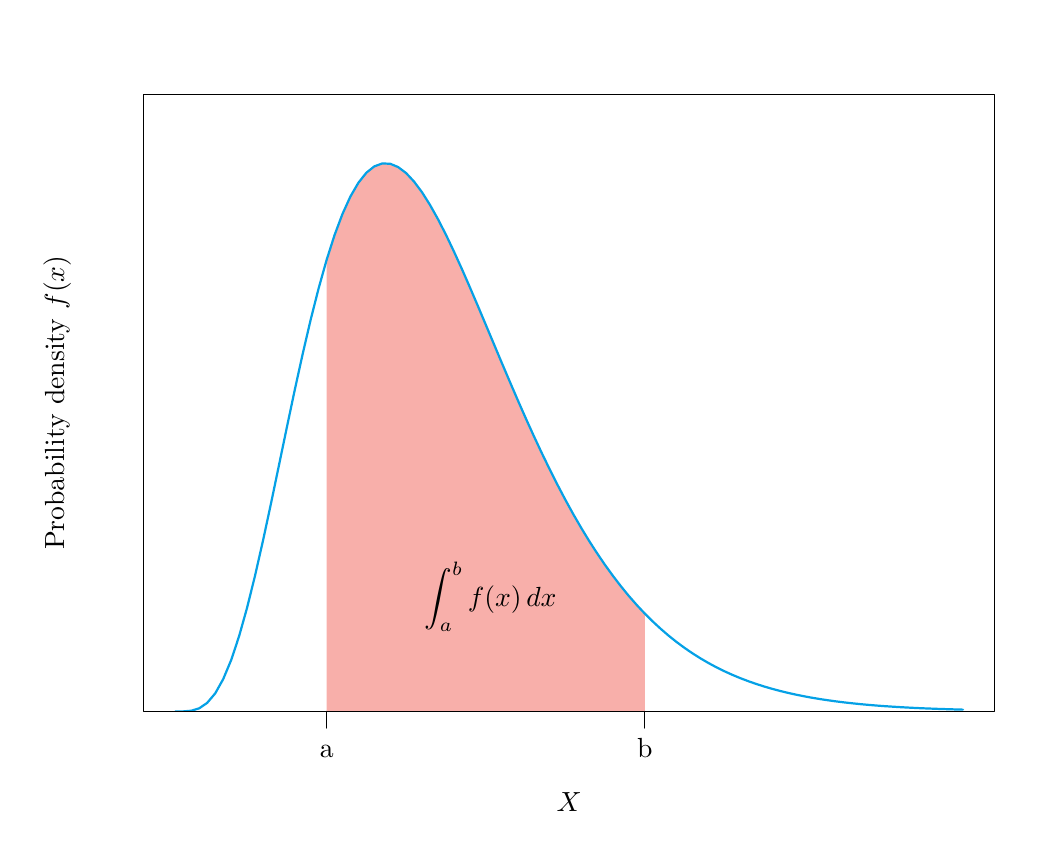
\begin{tikzpicture}[x=1pt,y=1pt]
\definecolor{fillColor}{RGB}{255,255,255}
\path[use as bounding box,fill=fillColor,fill opacity=0.00] (0,0) rectangle (361.35,289.08);
\begin{scope}
\path[clip] (  0.00,  0.00) rectangle (361.35,289.08);
\definecolor{drawColor}{RGB}{0,0,0}

\node[text=drawColor,anchor=base,inner sep=0pt, outer sep=0pt, scale=  1.00] at (195.67,  6.00) {$X$};

\node[text=drawColor,rotate= 90.00,anchor=base,inner sep=0pt, outer sep=0pt, scale=  1.00] at ( 13.20,153.54) {Probability density $f(x)$};
\end{scope}
\begin{scope}
\path[clip] (  0.00,  0.00) rectangle (361.35,289.08);
\definecolor{drawColor}{RGB}{0,0,0}

\path[draw=drawColor,line width= 0.4pt,line join=round,line cap=round] (108.00, 42.00) -- (222.98, 42.00);

\path[draw=drawColor,line width= 0.4pt,line join=round,line cap=round] (108.00, 42.00) -- (108.00, 36.00);

\path[draw=drawColor,line width= 0.4pt,line join=round,line cap=round] (222.98, 42.00) -- (222.98, 36.00);

\node[text=drawColor,anchor=base,inner sep=0pt, outer sep=0pt, scale=  1.00] at (108.00, 25.20) {a};

\node[text=drawColor,anchor=base,inner sep=0pt, outer sep=0pt, scale=  1.00] at (222.98, 25.20) {b};
\end{scope}
\begin{scope}
\path[clip] ( 42.00, 42.00) rectangle (349.35,265.08);
\definecolor{fillColor}{RGB}{238,50,36}

\path[fill=fillColor,fill opacity=0.39] (108.00, 42.00) --
	(108.00,205.09) --
	(110.87,214.08) --
	(113.75,221.76) --
	(116.62,228.08) --
	(119.50,233.03) --
	(122.37,236.65) --
	(125.25,238.95) --
	(128.12,240.01) --
	(131.00,239.90) --
	(133.87,238.71) --
	(136.75,236.53) --
	(139.62,233.46) --
	(142.50,229.60) --
	(145.37,225.05) --
	(148.24,219.92) --
	(151.12,214.30) --
	(153.99,208.28) --
	(156.87,201.95) --
	(159.74,195.38) --
	(162.62,188.66) --
	(165.49,181.84) --
	(168.37,174.99) --
	(171.24,168.15) --
	(174.12,161.39) --
	(176.99,154.73) --
	(179.86,148.21) --
	(182.74,141.86) --
	(185.61,135.71) --
	(188.49,129.77) --
	(191.36,124.06) --
	(194.24,118.58) --
	(197.11,113.35) --
	(199.99,108.38) --
	(202.86,103.65) --
	(205.74, 99.18) --
	(208.61, 94.96) --
	(211.49, 90.98) --
	(214.36, 87.24) --
	(217.23, 83.73) --
	(220.11, 80.44) --
	(222.98, 77.38) --
	(222.98, 42.00) --
	cycle;
\definecolor{drawColor}{RGB}{5,161,230}

\path[draw=drawColor,line width= 0.8pt,line join=round,line cap=round] ( 53.38, 42.00) --
	( 56.26, 42.02) --
	( 59.13, 42.26) --
	( 62.01, 43.14) --
	( 64.88, 45.11) --
	( 67.76, 48.52) --
	( 70.63, 53.63) --
	( 73.51, 60.51) --
	( 76.38, 69.14) --
	( 79.25, 79.36) --
	( 82.13, 90.94) --
	( 85.00,103.57) --
	( 87.88,116.95) --
	( 90.75,130.71) --
	( 93.63,144.55) --
	( 96.50,158.14) --
	( 99.38,171.21) --
	(102.25,183.52) --
	(105.13,194.86) --
	(108.00,205.09) --
	(110.87,214.08) --
	(113.75,221.76) --
	(116.62,228.08) --
	(119.50,233.03) --
	(122.37,236.65) --
	(125.25,238.95) --
	(128.12,240.01) --
	(131.00,239.90) --
	(133.87,238.71) --
	(136.75,236.53) --
	(139.62,233.46) --
	(142.50,229.60) --
	(145.37,225.05) --
	(148.24,219.92) --
	(151.12,214.30) --
	(153.99,208.28) --
	(156.87,201.95) --
	(159.74,195.38) --
	(162.62,188.66) --
	(165.49,181.84) --
	(168.37,174.99) --
	(171.24,168.15) --
	(174.12,161.39) --
	(176.99,154.73) --
	(179.86,148.21) --
	(182.74,141.86) --
	(185.61,135.71) --
	(188.49,129.77) --
	(191.36,124.06) --
	(194.24,118.58) --
	(197.11,113.35) --
	(199.99,108.38) --
	(202.86,103.65) --
	(205.74, 99.18) --
	(208.61, 94.96) --
	(211.49, 90.98) --
	(214.36, 87.24) --
	(217.23, 83.73) --
	(220.11, 80.44) --
	(222.98, 77.38) --
	(225.86, 74.52) --
	(228.73, 71.86) --
	(231.61, 69.38) --
	(234.48, 67.09) --
	(237.36, 64.96) --
	(240.23, 63.00) --
	(243.11, 61.18) --
	(245.98, 59.51) --
	(248.85, 57.96) --
	(251.73, 56.54) --
	(254.60, 55.24) --
	(257.48, 54.04) --
	(260.35, 52.95) --
	(263.23, 51.94) --
	(266.10, 51.02) --
	(268.98, 50.18) --
	(271.85, 49.41) --
	(274.73, 48.71) --
	(277.60, 48.07) --
	(280.48, 47.49) --
	(283.35, 46.96) --
	(286.22, 46.48) --
	(289.10, 46.05) --
	(291.97, 45.65) --
	(294.85, 45.29) --
	(297.72, 44.97) --
	(300.60, 44.67) --
	(303.47, 44.40) --
	(306.35, 44.16) --
	(309.22, 43.94) --
	(312.10, 43.75) --
	(314.97, 43.57) --
	(317.84, 43.41) --
	(320.72, 43.26) --
	(323.59, 43.13) --
	(326.47, 43.02) --
	(329.34, 42.91) --
	(332.22, 42.82) --
	(335.09, 42.73) --
	(337.97, 42.65);
\definecolor{drawColor}{RGB}{0,0,0}

\node[text=drawColor,anchor=base,inner sep=0pt, outer sep=0pt, scale=  1.00] at (167.22, 80.06) {$\displaystyle \int_a^b f(x)\,dx$};
\end{scope}
\begin{scope}
\path[clip] (  0.00,  0.00) rectangle (361.35,289.08);
\definecolor{drawColor}{RGB}{0,0,0}

\path[draw=drawColor,line width= 0.4pt,line join=round,line cap=round] ( 42.00, 42.00) --
	(349.35, 42.00) --
	(349.35,265.08) --
	( 42.00,265.08) --
	( 42.00, 42.00);
\end{scope}
\end{tikzpicture}
}}
$\displaystyle P(a\leq X\leq b) = \int_a^b f(x)\, dx = F(b)-F(a)$
\end{center}
\end{frame}



%---------------------------------------------------------------------slide----
\begin{frame}
\frametitle{Probability calculation}
\framesubtitle{Example}
Given the following function
\[
f(x) =
\begin{cases}
0 & \mbox{si $x<0$}\\
e^{-x} & \mbox{si $x\geq 0$},
\end{cases}
\]
let's check that is a density function. 

As this function is clearly non-negative, we have to check that total area bounded by the curve and the x-axis is 1.
\begin{align*}
\int_{-\infty}^\infty f(x)\;dx &= \int_{-\infty}^0 f(x)\;dx +\int_0^\infty f(x)\;dx = \int_{-\infty}^0 0\;dx +\int_0^\infty e^{-x}\;dx =\\
&= \left[-e^{-x}\right]_0^{\infty} = -e^{-\infty}+e^0 = 1.
\end{align*}
Now, let's calculate the probability of $X$ having a value between 0 and 2. 
\begin{align*}
P(0\leq X\leq 2) &= \int_0^2 f(x)\;dx = \int_0^2 e^{-x}\;dx = \left[-e^{-x}\right]_0^2 = -e^{-2}+e^0 = 0.8646.
\end{align*}
\end{frame}


%---------------------------------------------------------------------slide----
\begin{frame}
\frametitle{Population statistics}
The calculation of the population statistics is similar to the case of discrete variables, but using the density
function instead of the probability function, and extending the discrete sum to the integral.

The most important are:
\begin{itemize}
\item \structure{Mean}:
\[
\mu = E(X) = \int_{-\infty}^\infty x f(x)\; dx
\]
\item \structure{Variance}:
\[
\sigma^2 = Var(X) = \int_{-\infty}^\infty x^2f(x)\; dx -\mu^2
\]
\item \structure{Standard deviation}:
\[
\sigma = +\sqrt{\sigma^2}
\]
\end{itemize}
\end{frame}


%---------------------------------------------------------------------slide----
\begin{frame}
\frametitle{Population statistics}
\framesubtitle{Example}
Let $X$ be a variable with the following probability density function
\[
f(x) =
\begin{cases}
0 & \mbox{si $x<0$}\\
e^{-x} & \mbox{si $x\geq 0$}
\end{cases}
\]

The mean is 
\begin{align*}
\mu &= \int_{-\infty}^\infty xf(x)\;dx = \int_{-\infty}^0 xf(x)\;dx +\int_0^\infty xf(x)\;dx = \int_{-\infty}^0 0\;dx +\int_0^\infty xe^{-x}\;dx =\\
&= \left[-e^{-x}(1+x)\right]_0^{\infty} = 1.
\end{align*}
and the variance is
\begin{align*}
\sigma^2 &= \int_{-\infty}^\infty x^2f(x)\;dx -\mu^2 = \int_{-\infty}^0 x^2f(x)\;dx +\int_0^\infty x^2f(x)\;dx -\mu^2 = \\
&= \int_{-\infty}^0 0\;dx +\int_0^\infty x^2e^{-x}\;dx -\mu^2= \left[-e^{-x}(x^2+2x+2)\right]_0^{\infty} - 1^2= 2e^0-1 = 1.
\end{align*}
\end{frame}



%---------------------------------------------------------------------slide----
\begin{frame}
\frametitle{Continuous probability distribution models}
According to the type of experiment where the random variable is measured, there are different probability distributions
models. 
The most common are
\begin{itemize}
\item Continuous uniform.
\item Normal.
\item Student's T.
\item Chi-square.
\item Fisher-Snedecor's F.
\end{itemize}
\end{frame}


\subsection{Continuous uniform distribution}

%---------------------------------------------------------------------slide----
\begin{frame}
\frametitle{Continuous uniform probability distribution model $U(a,b)$}
When all the values of a random variable $X$ have equal probability, the probability distribution of $X$ is uniform.

\begin{definition}[Continuous uniform distribution $U(a,b)$]
A continuouo random variable $X$ follows a probability distribution model \emph{uniform} of parameters $a$ and
$b$, noted $X\sim U(a,b)$, if its range is $\mbox{Ran}(X) = [a,b]$ and its density function is
\[
f(x)= \frac{1}{b-a}\quad \forall x\in [a,b]
\]
\end{definition}

Observe that $a$ and $b$ are the minimum and the maximum of the range respectively, and that the density function is
constant. 

The mean and the variance are
\[
\mu = \frac{a+b}{2}\qquad \sigma^2=\frac{(b-a)^2}{12}.
\]
\end{frame}


%---------------------------------------------------------------------slide----
\begin{frame}
\frametitle{Continuous uniform probability density function}
\framesubtitle{Example}

The generation of a random number between 0 and 1 is follows a continuous uniform distribution $U(0,1)$.
\begin{center}
\tikzsetnextfilename{continuous_random_variables/uniform_density_function}
\mode<article>{\resizebox{0.7\textwidth}{!}{% Created by tikzDevice version 0.9 on 2016-04-28 17:31:47
% !TEX encoding = UTF-8 Unicode
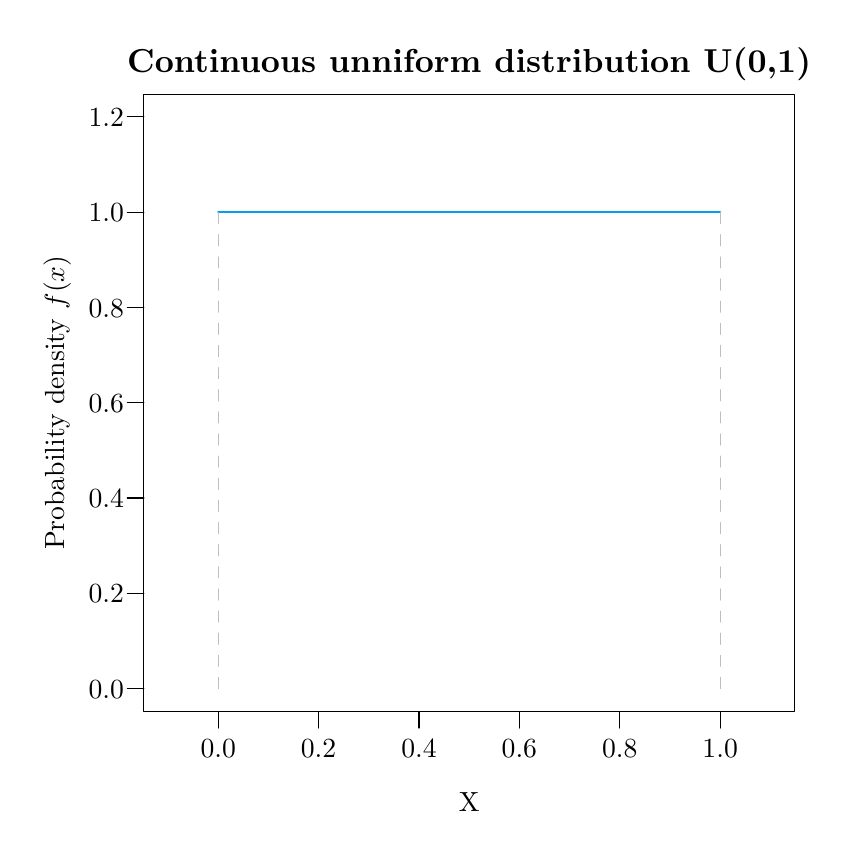
\begin{tikzpicture}[x=1pt,y=1pt]
\definecolor{fillColor}{RGB}{255,255,255}
\path[use as bounding box,fill=fillColor,fill opacity=0.00] (0,0) rectangle (289.08,289.08);
\begin{scope}
\path[clip] ( 42.00, 42.00) rectangle (277.08,265.08);
\definecolor{drawColor}{RGB}{5,161,230}

\path[draw=drawColor,line width= 0.8pt,line join=round,line cap=round] ( 68.85,222.39) --
	( 89.00,222.39) --
	(109.15,222.39) --
	(129.31,222.39) --
	(149.46,222.39) --
	(169.62,222.39) --
	(189.77,222.39) --
	(209.93,222.39) --
	(230.08,222.39) --
	(250.23,222.39);
\end{scope}
\begin{scope}
\path[clip] (  0.00,  0.00) rectangle (289.08,289.08);
\definecolor{drawColor}{RGB}{0,0,0}

\path[draw=drawColor,line width= 0.4pt,line join=round,line cap=round] ( 68.85, 42.00) -- (250.23, 42.00);

\path[draw=drawColor,line width= 0.4pt,line join=round,line cap=round] ( 68.85, 42.00) -- ( 68.85, 36.00);

\path[draw=drawColor,line width= 0.4pt,line join=round,line cap=round] (105.12, 42.00) -- (105.12, 36.00);

\path[draw=drawColor,line width= 0.4pt,line join=round,line cap=round] (141.40, 42.00) -- (141.40, 36.00);

\path[draw=drawColor,line width= 0.4pt,line join=round,line cap=round] (177.68, 42.00) -- (177.68, 36.00);

\path[draw=drawColor,line width= 0.4pt,line join=round,line cap=round] (213.96, 42.00) -- (213.96, 36.00);

\path[draw=drawColor,line width= 0.4pt,line join=round,line cap=round] (250.23, 42.00) -- (250.23, 36.00);

\node[text=drawColor,anchor=base,inner sep=0pt, outer sep=0pt, scale=  1.00] at ( 68.85, 25.20) {0.0};

\node[text=drawColor,anchor=base,inner sep=0pt, outer sep=0pt, scale=  1.00] at (105.12, 25.20) {0.2};

\node[text=drawColor,anchor=base,inner sep=0pt, outer sep=0pt, scale=  1.00] at (141.40, 25.20) {0.4};

\node[text=drawColor,anchor=base,inner sep=0pt, outer sep=0pt, scale=  1.00] at (177.68, 25.20) {0.6};

\node[text=drawColor,anchor=base,inner sep=0pt, outer sep=0pt, scale=  1.00] at (213.96, 25.20) {0.8};

\node[text=drawColor,anchor=base,inner sep=0pt, outer sep=0pt, scale=  1.00] at (250.23, 25.20) {1.0};

\path[draw=drawColor,line width= 0.4pt,line join=round,line cap=round] ( 42.00, 50.26) -- ( 42.00,256.82);

\path[draw=drawColor,line width= 0.4pt,line join=round,line cap=round] ( 42.00, 50.26) -- ( 36.00, 50.26);

\path[draw=drawColor,line width= 0.4pt,line join=round,line cap=round] ( 42.00, 84.69) -- ( 36.00, 84.69);

\path[draw=drawColor,line width= 0.4pt,line join=round,line cap=round] ( 42.00,119.11) -- ( 36.00,119.11);

\path[draw=drawColor,line width= 0.4pt,line join=round,line cap=round] ( 42.00,153.54) -- ( 36.00,153.54);

\path[draw=drawColor,line width= 0.4pt,line join=round,line cap=round] ( 42.00,187.97) -- ( 36.00,187.97);

\path[draw=drawColor,line width= 0.4pt,line join=round,line cap=round] ( 42.00,222.39) -- ( 36.00,222.39);

\path[draw=drawColor,line width= 0.4pt,line join=round,line cap=round] ( 42.00,256.82) -- ( 36.00,256.82);

\node[text=drawColor,anchor=base east,inner sep=0pt, outer sep=0pt, scale=  1.00] at ( 34.80, 46.82) {0.0};

\node[text=drawColor,anchor=base east,inner sep=0pt, outer sep=0pt, scale=  1.00] at ( 34.80, 81.24) {0.2};

\node[text=drawColor,anchor=base east,inner sep=0pt, outer sep=0pt, scale=  1.00] at ( 34.80,115.67) {0.4};

\node[text=drawColor,anchor=base east,inner sep=0pt, outer sep=0pt, scale=  1.00] at ( 34.80,150.10) {0.6};

\node[text=drawColor,anchor=base east,inner sep=0pt, outer sep=0pt, scale=  1.00] at ( 34.80,184.52) {0.8};

\node[text=drawColor,anchor=base east,inner sep=0pt, outer sep=0pt, scale=  1.00] at ( 34.80,218.95) {1.0};

\node[text=drawColor,anchor=base east,inner sep=0pt, outer sep=0pt, scale=  1.00] at ( 34.80,253.37) {1.2};

\path[draw=drawColor,line width= 0.4pt,line join=round,line cap=round] ( 42.00, 42.00) --
	(277.08, 42.00) --
	(277.08,265.08) --
	( 42.00,265.08) --
	( 42.00, 42.00);
\end{scope}
\begin{scope}
\path[clip] (  0.00,  0.00) rectangle (289.08,289.08);
\definecolor{drawColor}{RGB}{0,0,0}

\node[text=drawColor,anchor=base,inner sep=0pt, outer sep=0pt, scale=  1.20] at (159.54,272.89) {\bfseries Continuous unniform distribution U(0,1)};

\node[text=drawColor,anchor=base,inner sep=0pt, outer sep=0pt, scale=  1.00] at (159.54,  6.00) {X};

\node[text=drawColor,rotate= 90.00,anchor=base,inner sep=0pt, outer sep=0pt, scale=  1.00] at ( 13.20,153.54) {Probability density $f(x)$};
\end{scope}
\begin{scope}
\path[clip] ( 42.00, 42.00) rectangle (277.08,265.08);
\definecolor{drawColor}{RGB}{190,190,190}

\path[draw=drawColor,line width= 0.4pt,dash pattern=on 4pt off 4pt ,line join=round,line cap=round] ( 68.85, 50.26) -- ( 68.85,222.39);

\path[draw=drawColor,line width= 0.4pt,dash pattern=on 4pt off 4pt ,line join=round,line cap=round] (250.23, 50.26) -- (250.23,222.39);
\end{scope}
\end{tikzpicture}
}}
\mode<presentation>{\resizebox{0.6\textwidth}{!}{% Created by tikzDevice version 0.9 on 2016-04-28 17:31:47
% !TEX encoding = UTF-8 Unicode
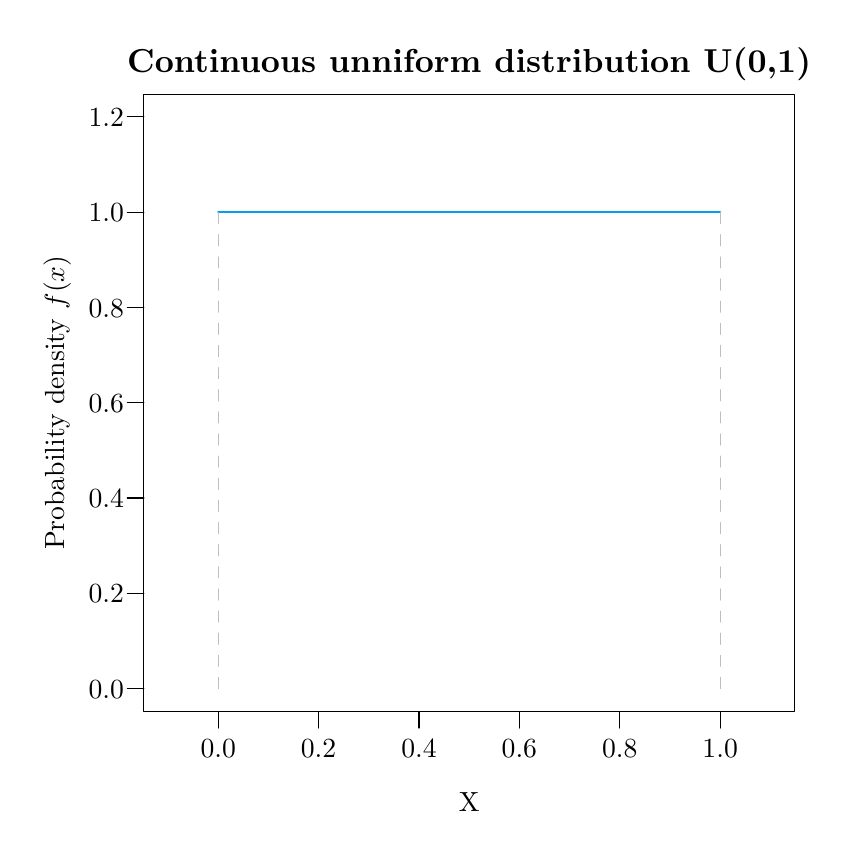
\begin{tikzpicture}[x=1pt,y=1pt]
\definecolor{fillColor}{RGB}{255,255,255}
\path[use as bounding box,fill=fillColor,fill opacity=0.00] (0,0) rectangle (289.08,289.08);
\begin{scope}
\path[clip] ( 42.00, 42.00) rectangle (277.08,265.08);
\definecolor{drawColor}{RGB}{5,161,230}

\path[draw=drawColor,line width= 0.8pt,line join=round,line cap=round] ( 68.85,222.39) --
	( 89.00,222.39) --
	(109.15,222.39) --
	(129.31,222.39) --
	(149.46,222.39) --
	(169.62,222.39) --
	(189.77,222.39) --
	(209.93,222.39) --
	(230.08,222.39) --
	(250.23,222.39);
\end{scope}
\begin{scope}
\path[clip] (  0.00,  0.00) rectangle (289.08,289.08);
\definecolor{drawColor}{RGB}{0,0,0}

\path[draw=drawColor,line width= 0.4pt,line join=round,line cap=round] ( 68.85, 42.00) -- (250.23, 42.00);

\path[draw=drawColor,line width= 0.4pt,line join=round,line cap=round] ( 68.85, 42.00) -- ( 68.85, 36.00);

\path[draw=drawColor,line width= 0.4pt,line join=round,line cap=round] (105.12, 42.00) -- (105.12, 36.00);

\path[draw=drawColor,line width= 0.4pt,line join=round,line cap=round] (141.40, 42.00) -- (141.40, 36.00);

\path[draw=drawColor,line width= 0.4pt,line join=round,line cap=round] (177.68, 42.00) -- (177.68, 36.00);

\path[draw=drawColor,line width= 0.4pt,line join=round,line cap=round] (213.96, 42.00) -- (213.96, 36.00);

\path[draw=drawColor,line width= 0.4pt,line join=round,line cap=round] (250.23, 42.00) -- (250.23, 36.00);

\node[text=drawColor,anchor=base,inner sep=0pt, outer sep=0pt, scale=  1.00] at ( 68.85, 25.20) {0.0};

\node[text=drawColor,anchor=base,inner sep=0pt, outer sep=0pt, scale=  1.00] at (105.12, 25.20) {0.2};

\node[text=drawColor,anchor=base,inner sep=0pt, outer sep=0pt, scale=  1.00] at (141.40, 25.20) {0.4};

\node[text=drawColor,anchor=base,inner sep=0pt, outer sep=0pt, scale=  1.00] at (177.68, 25.20) {0.6};

\node[text=drawColor,anchor=base,inner sep=0pt, outer sep=0pt, scale=  1.00] at (213.96, 25.20) {0.8};

\node[text=drawColor,anchor=base,inner sep=0pt, outer sep=0pt, scale=  1.00] at (250.23, 25.20) {1.0};

\path[draw=drawColor,line width= 0.4pt,line join=round,line cap=round] ( 42.00, 50.26) -- ( 42.00,256.82);

\path[draw=drawColor,line width= 0.4pt,line join=round,line cap=round] ( 42.00, 50.26) -- ( 36.00, 50.26);

\path[draw=drawColor,line width= 0.4pt,line join=round,line cap=round] ( 42.00, 84.69) -- ( 36.00, 84.69);

\path[draw=drawColor,line width= 0.4pt,line join=round,line cap=round] ( 42.00,119.11) -- ( 36.00,119.11);

\path[draw=drawColor,line width= 0.4pt,line join=round,line cap=round] ( 42.00,153.54) -- ( 36.00,153.54);

\path[draw=drawColor,line width= 0.4pt,line join=round,line cap=round] ( 42.00,187.97) -- ( 36.00,187.97);

\path[draw=drawColor,line width= 0.4pt,line join=round,line cap=round] ( 42.00,222.39) -- ( 36.00,222.39);

\path[draw=drawColor,line width= 0.4pt,line join=round,line cap=round] ( 42.00,256.82) -- ( 36.00,256.82);

\node[text=drawColor,anchor=base east,inner sep=0pt, outer sep=0pt, scale=  1.00] at ( 34.80, 46.82) {0.0};

\node[text=drawColor,anchor=base east,inner sep=0pt, outer sep=0pt, scale=  1.00] at ( 34.80, 81.24) {0.2};

\node[text=drawColor,anchor=base east,inner sep=0pt, outer sep=0pt, scale=  1.00] at ( 34.80,115.67) {0.4};

\node[text=drawColor,anchor=base east,inner sep=0pt, outer sep=0pt, scale=  1.00] at ( 34.80,150.10) {0.6};

\node[text=drawColor,anchor=base east,inner sep=0pt, outer sep=0pt, scale=  1.00] at ( 34.80,184.52) {0.8};

\node[text=drawColor,anchor=base east,inner sep=0pt, outer sep=0pt, scale=  1.00] at ( 34.80,218.95) {1.0};

\node[text=drawColor,anchor=base east,inner sep=0pt, outer sep=0pt, scale=  1.00] at ( 34.80,253.37) {1.2};

\path[draw=drawColor,line width= 0.4pt,line join=round,line cap=round] ( 42.00, 42.00) --
	(277.08, 42.00) --
	(277.08,265.08) --
	( 42.00,265.08) --
	( 42.00, 42.00);
\end{scope}
\begin{scope}
\path[clip] (  0.00,  0.00) rectangle (289.08,289.08);
\definecolor{drawColor}{RGB}{0,0,0}

\node[text=drawColor,anchor=base,inner sep=0pt, outer sep=0pt, scale=  1.20] at (159.54,272.89) {\bfseries Continuous unniform distribution U(0,1)};

\node[text=drawColor,anchor=base,inner sep=0pt, outer sep=0pt, scale=  1.00] at (159.54,  6.00) {X};

\node[text=drawColor,rotate= 90.00,anchor=base,inner sep=0pt, outer sep=0pt, scale=  1.00] at ( 13.20,153.54) {Probability density $f(x)$};
\end{scope}
\begin{scope}
\path[clip] ( 42.00, 42.00) rectangle (277.08,265.08);
\definecolor{drawColor}{RGB}{190,190,190}

\path[draw=drawColor,line width= 0.4pt,dash pattern=on 4pt off 4pt ,line join=round,line cap=round] ( 68.85, 50.26) -- ( 68.85,222.39);

\path[draw=drawColor,line width= 0.4pt,dash pattern=on 4pt off 4pt ,line join=round,line cap=round] (250.23, 50.26) -- (250.23,222.39);
\end{scope}
\end{tikzpicture}
}}
\end{center}
\end{frame}


%---------------------------------------------------------------------slide----
\begin{frame}
\frametitle{Continuous uniform distribution function}
\framesubtitle{Example}
As the density function is constant, the distribution function has a linear growth. 
\begin{center}
\tikzsetnextfilename{continuous_random_variables/uniform_distribution_function}
\mode<article>{\resizebox{0.7\textwidth}{!}{% Created by tikzDevice version 0.9 on 2016-04-28 17:47:04
% !TEX encoding = UTF-8 Unicode
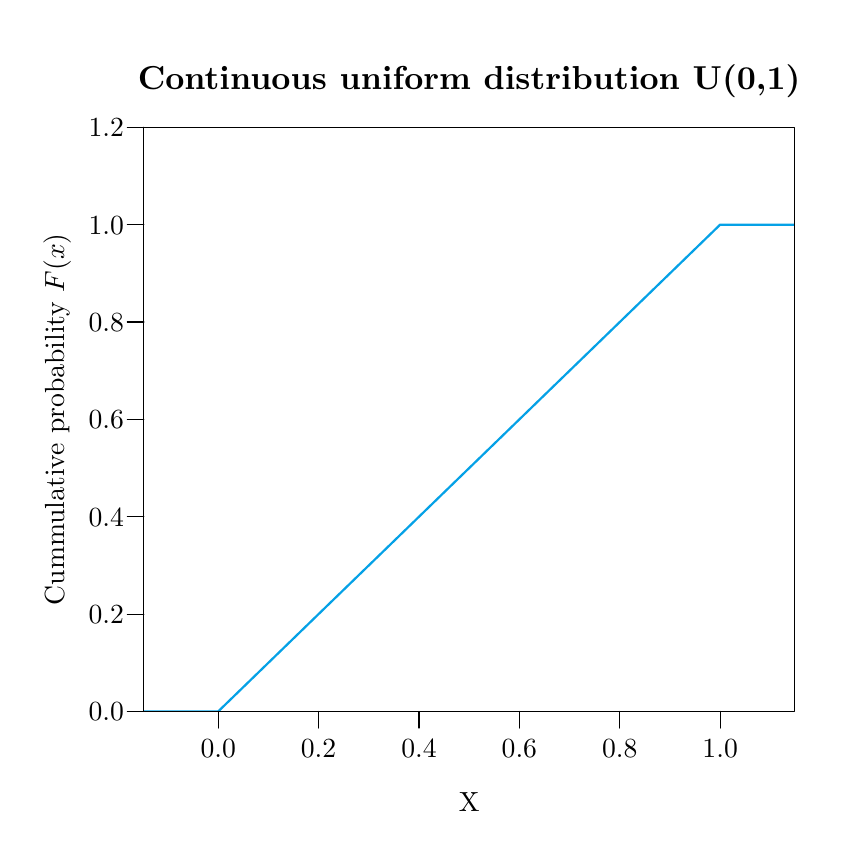
\begin{tikzpicture}[x=1pt,y=1pt]
\definecolor{fillColor}{RGB}{255,255,255}
\path[use as bounding box,fill=fillColor,fill opacity=0.00] (0,0) rectangle (289.08,289.08);
\begin{scope}
\path[clip] ( 42.00, 42.00) rectangle (277.08,253.08);
\definecolor{drawColor}{RGB}{5,161,230}

\path[draw=drawColor,line width= 0.8pt,line join=round,line cap=round] ( 32.57, 42.00) --
	( 68.85, 42.00) --
	( 89.00, 61.54) --
	(109.15, 81.09) --
	(129.31,100.63) --
	(149.46,120.18) --
	(169.62,139.72) --
	(189.77,159.27) --
	(209.93,178.81) --
	(230.08,198.36) --
	(250.23,217.90) --
	(286.51,217.90);
\end{scope}
\begin{scope}
\path[clip] (  0.00,  0.00) rectangle (289.08,289.08);
\definecolor{drawColor}{RGB}{0,0,0}

\path[draw=drawColor,line width= 0.4pt,line join=round,line cap=round] ( 68.85, 42.00) -- (250.23, 42.00);

\path[draw=drawColor,line width= 0.4pt,line join=round,line cap=round] ( 68.85, 42.00) -- ( 68.85, 36.00);

\path[draw=drawColor,line width= 0.4pt,line join=round,line cap=round] (105.12, 42.00) -- (105.12, 36.00);

\path[draw=drawColor,line width= 0.4pt,line join=round,line cap=round] (141.40, 42.00) -- (141.40, 36.00);

\path[draw=drawColor,line width= 0.4pt,line join=round,line cap=round] (177.68, 42.00) -- (177.68, 36.00);

\path[draw=drawColor,line width= 0.4pt,line join=round,line cap=round] (213.96, 42.00) -- (213.96, 36.00);

\path[draw=drawColor,line width= 0.4pt,line join=round,line cap=round] (250.23, 42.00) -- (250.23, 36.00);

\node[text=drawColor,anchor=base,inner sep=0pt, outer sep=0pt, scale=  1.00] at ( 68.85, 25.20) {0.0};

\node[text=drawColor,anchor=base,inner sep=0pt, outer sep=0pt, scale=  1.00] at (105.12, 25.20) {0.2};

\node[text=drawColor,anchor=base,inner sep=0pt, outer sep=0pt, scale=  1.00] at (141.40, 25.20) {0.4};

\node[text=drawColor,anchor=base,inner sep=0pt, outer sep=0pt, scale=  1.00] at (177.68, 25.20) {0.6};

\node[text=drawColor,anchor=base,inner sep=0pt, outer sep=0pt, scale=  1.00] at (213.96, 25.20) {0.8};

\node[text=drawColor,anchor=base,inner sep=0pt, outer sep=0pt, scale=  1.00] at (250.23, 25.20) {1.0};

\path[draw=drawColor,line width= 0.4pt,line join=round,line cap=round] ( 42.00, 42.00) -- ( 42.00,253.08);

\path[draw=drawColor,line width= 0.4pt,line join=round,line cap=round] ( 42.00, 42.00) -- ( 36.00, 42.00);

\path[draw=drawColor,line width= 0.4pt,line join=round,line cap=round] ( 42.00, 77.18) -- ( 36.00, 77.18);

\path[draw=drawColor,line width= 0.4pt,line join=round,line cap=round] ( 42.00,112.36) -- ( 36.00,112.36);

\path[draw=drawColor,line width= 0.4pt,line join=round,line cap=round] ( 42.00,147.54) -- ( 36.00,147.54);

\path[draw=drawColor,line width= 0.4pt,line join=round,line cap=round] ( 42.00,182.72) -- ( 36.00,182.72);

\path[draw=drawColor,line width= 0.4pt,line join=round,line cap=round] ( 42.00,217.90) -- ( 36.00,217.90);

\path[draw=drawColor,line width= 0.4pt,line join=round,line cap=round] ( 42.00,253.08) -- ( 36.00,253.08);

\node[text=drawColor,anchor=base east,inner sep=0pt, outer sep=0pt, scale=  1.00] at ( 34.80, 38.56) {0.0};

\node[text=drawColor,anchor=base east,inner sep=0pt, outer sep=0pt, scale=  1.00] at ( 34.80, 73.74) {0.2};

\node[text=drawColor,anchor=base east,inner sep=0pt, outer sep=0pt, scale=  1.00] at ( 34.80,108.92) {0.4};

\node[text=drawColor,anchor=base east,inner sep=0pt, outer sep=0pt, scale=  1.00] at ( 34.80,144.10) {0.6};

\node[text=drawColor,anchor=base east,inner sep=0pt, outer sep=0pt, scale=  1.00] at ( 34.80,179.28) {0.8};

\node[text=drawColor,anchor=base east,inner sep=0pt, outer sep=0pt, scale=  1.00] at ( 34.80,214.46) {1.0};

\node[text=drawColor,anchor=base east,inner sep=0pt, outer sep=0pt, scale=  1.00] at ( 34.80,249.64) {1.2};

\path[draw=drawColor,line width= 0.4pt,line join=round,line cap=round] ( 42.00, 42.00) --
	(277.08, 42.00) --
	(277.08,253.08) --
	( 42.00,253.08) --
	( 42.00, 42.00);
\end{scope}
\begin{scope}
\path[clip] (  0.00,  0.00) rectangle (289.08,289.08);
\definecolor{drawColor}{RGB}{0,0,0}

\node[text=drawColor,anchor=base,inner sep=0pt, outer sep=0pt, scale=  1.20] at (159.54,266.89) {\bfseries Continuous uniform distribution U(0,1)};

\node[text=drawColor,anchor=base,inner sep=0pt, outer sep=0pt, scale=  1.00] at (159.54,  6.00) {X};

\node[text=drawColor,rotate= 90.00,anchor=base,inner sep=0pt, outer sep=0pt, scale=  1.00] at ( 13.20,147.54) {Cummulative probability $F(x)$};
\end{scope}
\end{tikzpicture}
}}
\mode<presentation>{\resizebox{0.6\textwidth}{!}{% Created by tikzDevice version 0.9 on 2016-04-28 17:47:04
% !TEX encoding = UTF-8 Unicode
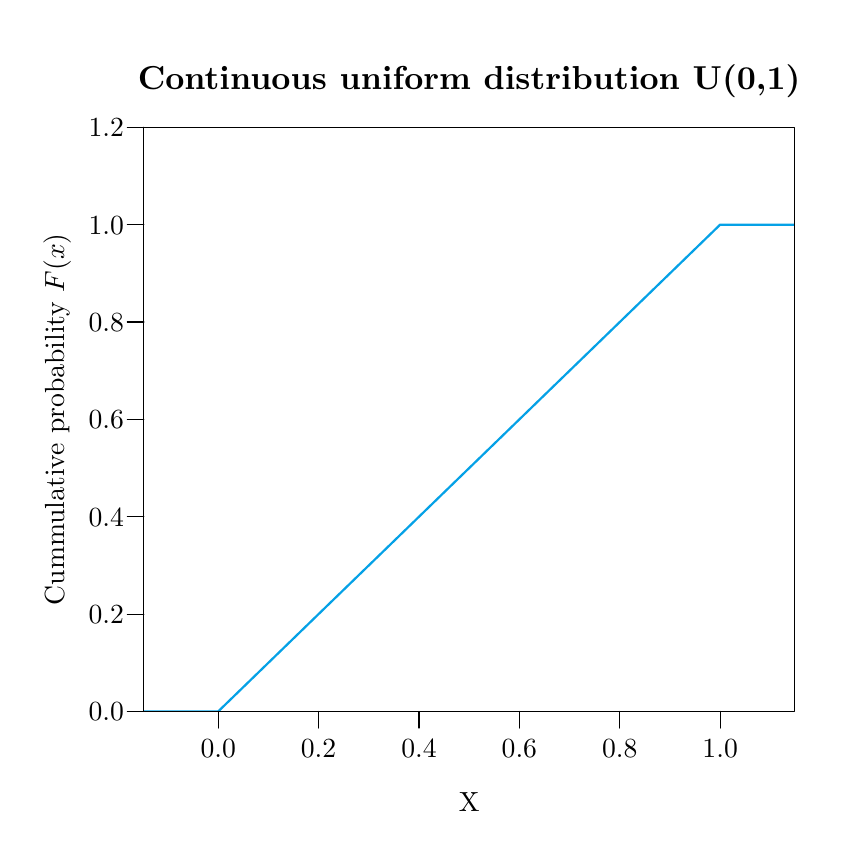
\begin{tikzpicture}[x=1pt,y=1pt]
\definecolor{fillColor}{RGB}{255,255,255}
\path[use as bounding box,fill=fillColor,fill opacity=0.00] (0,0) rectangle (289.08,289.08);
\begin{scope}
\path[clip] ( 42.00, 42.00) rectangle (277.08,253.08);
\definecolor{drawColor}{RGB}{5,161,230}

\path[draw=drawColor,line width= 0.8pt,line join=round,line cap=round] ( 32.57, 42.00) --
	( 68.85, 42.00) --
	( 89.00, 61.54) --
	(109.15, 81.09) --
	(129.31,100.63) --
	(149.46,120.18) --
	(169.62,139.72) --
	(189.77,159.27) --
	(209.93,178.81) --
	(230.08,198.36) --
	(250.23,217.90) --
	(286.51,217.90);
\end{scope}
\begin{scope}
\path[clip] (  0.00,  0.00) rectangle (289.08,289.08);
\definecolor{drawColor}{RGB}{0,0,0}

\path[draw=drawColor,line width= 0.4pt,line join=round,line cap=round] ( 68.85, 42.00) -- (250.23, 42.00);

\path[draw=drawColor,line width= 0.4pt,line join=round,line cap=round] ( 68.85, 42.00) -- ( 68.85, 36.00);

\path[draw=drawColor,line width= 0.4pt,line join=round,line cap=round] (105.12, 42.00) -- (105.12, 36.00);

\path[draw=drawColor,line width= 0.4pt,line join=round,line cap=round] (141.40, 42.00) -- (141.40, 36.00);

\path[draw=drawColor,line width= 0.4pt,line join=round,line cap=round] (177.68, 42.00) -- (177.68, 36.00);

\path[draw=drawColor,line width= 0.4pt,line join=round,line cap=round] (213.96, 42.00) -- (213.96, 36.00);

\path[draw=drawColor,line width= 0.4pt,line join=round,line cap=round] (250.23, 42.00) -- (250.23, 36.00);

\node[text=drawColor,anchor=base,inner sep=0pt, outer sep=0pt, scale=  1.00] at ( 68.85, 25.20) {0.0};

\node[text=drawColor,anchor=base,inner sep=0pt, outer sep=0pt, scale=  1.00] at (105.12, 25.20) {0.2};

\node[text=drawColor,anchor=base,inner sep=0pt, outer sep=0pt, scale=  1.00] at (141.40, 25.20) {0.4};

\node[text=drawColor,anchor=base,inner sep=0pt, outer sep=0pt, scale=  1.00] at (177.68, 25.20) {0.6};

\node[text=drawColor,anchor=base,inner sep=0pt, outer sep=0pt, scale=  1.00] at (213.96, 25.20) {0.8};

\node[text=drawColor,anchor=base,inner sep=0pt, outer sep=0pt, scale=  1.00] at (250.23, 25.20) {1.0};

\path[draw=drawColor,line width= 0.4pt,line join=round,line cap=round] ( 42.00, 42.00) -- ( 42.00,253.08);

\path[draw=drawColor,line width= 0.4pt,line join=round,line cap=round] ( 42.00, 42.00) -- ( 36.00, 42.00);

\path[draw=drawColor,line width= 0.4pt,line join=round,line cap=round] ( 42.00, 77.18) -- ( 36.00, 77.18);

\path[draw=drawColor,line width= 0.4pt,line join=round,line cap=round] ( 42.00,112.36) -- ( 36.00,112.36);

\path[draw=drawColor,line width= 0.4pt,line join=round,line cap=round] ( 42.00,147.54) -- ( 36.00,147.54);

\path[draw=drawColor,line width= 0.4pt,line join=round,line cap=round] ( 42.00,182.72) -- ( 36.00,182.72);

\path[draw=drawColor,line width= 0.4pt,line join=round,line cap=round] ( 42.00,217.90) -- ( 36.00,217.90);

\path[draw=drawColor,line width= 0.4pt,line join=round,line cap=round] ( 42.00,253.08) -- ( 36.00,253.08);

\node[text=drawColor,anchor=base east,inner sep=0pt, outer sep=0pt, scale=  1.00] at ( 34.80, 38.56) {0.0};

\node[text=drawColor,anchor=base east,inner sep=0pt, outer sep=0pt, scale=  1.00] at ( 34.80, 73.74) {0.2};

\node[text=drawColor,anchor=base east,inner sep=0pt, outer sep=0pt, scale=  1.00] at ( 34.80,108.92) {0.4};

\node[text=drawColor,anchor=base east,inner sep=0pt, outer sep=0pt, scale=  1.00] at ( 34.80,144.10) {0.6};

\node[text=drawColor,anchor=base east,inner sep=0pt, outer sep=0pt, scale=  1.00] at ( 34.80,179.28) {0.8};

\node[text=drawColor,anchor=base east,inner sep=0pt, outer sep=0pt, scale=  1.00] at ( 34.80,214.46) {1.0};

\node[text=drawColor,anchor=base east,inner sep=0pt, outer sep=0pt, scale=  1.00] at ( 34.80,249.64) {1.2};

\path[draw=drawColor,line width= 0.4pt,line join=round,line cap=round] ( 42.00, 42.00) --
	(277.08, 42.00) --
	(277.08,253.08) --
	( 42.00,253.08) --
	( 42.00, 42.00);
\end{scope}
\begin{scope}
\path[clip] (  0.00,  0.00) rectangle (289.08,289.08);
\definecolor{drawColor}{RGB}{0,0,0}

\node[text=drawColor,anchor=base,inner sep=0pt, outer sep=0pt, scale=  1.20] at (159.54,266.89) {\bfseries Continuous uniform distribution U(0,1)};

\node[text=drawColor,anchor=base,inner sep=0pt, outer sep=0pt, scale=  1.00] at (159.54,  6.00) {X};

\node[text=drawColor,rotate= 90.00,anchor=base,inner sep=0pt, outer sep=0pt, scale=  1.00] at ( 13.20,147.54) {Cummulative probability $F(x)$};
\end{scope}
\end{tikzpicture}
}}
\end{center}
\end{frame}


% ---------------------------------------------------------------------slide----
\begin{frame}
\frametitle{Cálculo de probabilidades con una Uniforme continua}
\framesubtitle{Ejemplo de espera de un autobús}
Supóngase que un autobús pasa por una parada cada 15 minutos. Si una persona puede llegar a la parada en cualquier instante, \emph{¿cuál es
la probabilidad de que espere entre 5 y 10 minutos?}
\begin{columns}
\begin{column}{0.52\textwidth}
En este caso, la variable $X$ que mide el tiempo de espera sigue un modelo de distribución uniforme continua $U(0,15)$ ya que cualquier
valor entre los 0 y los 15 minutos es equipobrable.

Así pues, la probabilidad que nos piden es
\begin{align*}
P(5\leq X\leq 10) &= \int_{5}^{10} \frac{1}{15}\;dx = \left[\frac{x}{15}\right]_5^{10} = \\
&= \frac{10}{15}-\frac{5}{15} =\frac{1}{3}.
\end{align*}
\end{column}
\begin{column}{0.43\textwidth}
\begin{center}
\tikzsetnextfilename{continuous_random_variables/uniform_probability_calculation}
\mode<article>{\resizebox{0.7\textwidth}{!}{% Created by tikzDevice version 0.9 on 2016-04-29 13:16:45
% !TEX encoding = UTF-8 Unicode
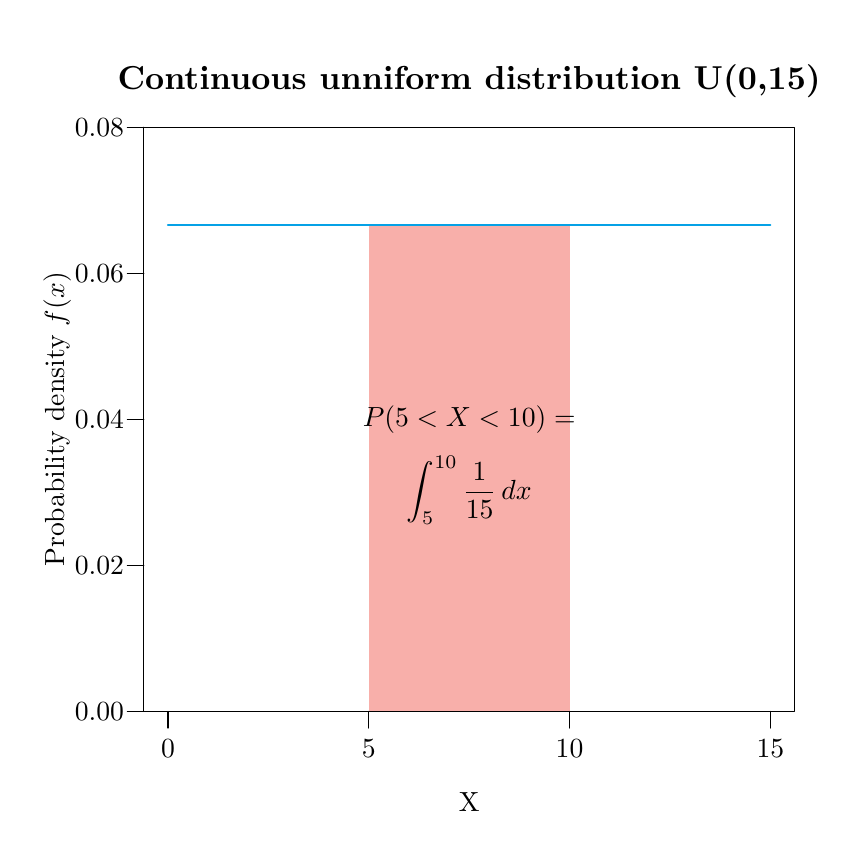
\begin{tikzpicture}[x=1pt,y=1pt]
\definecolor{fillColor}{RGB}{255,255,255}
\path[use as bounding box,fill=fillColor,fill opacity=0.00] (0,0) rectangle (289.08,289.08);
\begin{scope}
\path[clip] (  0.00,  0.00) rectangle (289.08,289.08);
\definecolor{drawColor}{RGB}{0,0,0}

\path[draw=drawColor,line width= 0.4pt,line join=round,line cap=round] ( 50.71, 42.00) -- (268.37, 42.00);

\path[draw=drawColor,line width= 0.4pt,line join=round,line cap=round] ( 50.71, 42.00) -- ( 50.71, 36.00);

\path[draw=drawColor,line width= 0.4pt,line join=round,line cap=round] (123.26, 42.00) -- (123.26, 36.00);

\path[draw=drawColor,line width= 0.4pt,line join=round,line cap=round] (195.82, 42.00) -- (195.82, 36.00);

\path[draw=drawColor,line width= 0.4pt,line join=round,line cap=round] (268.37, 42.00) -- (268.37, 36.00);

\node[text=drawColor,anchor=base,inner sep=0pt, outer sep=0pt, scale=  1.00] at ( 50.71, 25.20) {0};

\node[text=drawColor,anchor=base,inner sep=0pt, outer sep=0pt, scale=  1.00] at (123.26, 25.20) {5};

\node[text=drawColor,anchor=base,inner sep=0pt, outer sep=0pt, scale=  1.00] at (195.82, 25.20) {10};

\node[text=drawColor,anchor=base,inner sep=0pt, outer sep=0pt, scale=  1.00] at (268.37, 25.20) {15};

\path[draw=drawColor,line width= 0.4pt,line join=round,line cap=round] ( 42.00, 42.00) -- ( 42.00,253.08);

\path[draw=drawColor,line width= 0.4pt,line join=round,line cap=round] ( 42.00, 42.00) -- ( 36.00, 42.00);

\path[draw=drawColor,line width= 0.4pt,line join=round,line cap=round] ( 42.00, 94.77) -- ( 36.00, 94.77);

\path[draw=drawColor,line width= 0.4pt,line join=round,line cap=round] ( 42.00,147.54) -- ( 36.00,147.54);

\path[draw=drawColor,line width= 0.4pt,line join=round,line cap=round] ( 42.00,200.31) -- ( 36.00,200.31);

\path[draw=drawColor,line width= 0.4pt,line join=round,line cap=round] ( 42.00,253.08) -- ( 36.00,253.08);

\node[text=drawColor,anchor=base east,inner sep=0pt, outer sep=0pt, scale=  1.00] at ( 34.80, 38.56) {0.00};

\node[text=drawColor,anchor=base east,inner sep=0pt, outer sep=0pt, scale=  1.00] at ( 34.80, 91.33) {0.02};

\node[text=drawColor,anchor=base east,inner sep=0pt, outer sep=0pt, scale=  1.00] at ( 34.80,144.10) {0.04};

\node[text=drawColor,anchor=base east,inner sep=0pt, outer sep=0pt, scale=  1.00] at ( 34.80,196.87) {0.06};

\node[text=drawColor,anchor=base east,inner sep=0pt, outer sep=0pt, scale=  1.00] at ( 34.80,249.64) {0.08};

\path[draw=drawColor,line width= 0.4pt,line join=round,line cap=round] ( 42.00, 42.00) --
	(277.08, 42.00) --
	(277.08,253.08) --
	( 42.00,253.08) --
	( 42.00, 42.00);
\end{scope}
\begin{scope}
\path[clip] (  0.00,  0.00) rectangle (289.08,289.08);
\definecolor{drawColor}{RGB}{0,0,0}

\node[text=drawColor,anchor=base,inner sep=0pt, outer sep=0pt, scale=  1.20] at (159.54,266.89) {\bfseries Continuous unniform distribution U(0,15)};

\node[text=drawColor,anchor=base,inner sep=0pt, outer sep=0pt, scale=  1.00] at (159.54,  6.00) {X};

\node[text=drawColor,rotate= 90.00,anchor=base,inner sep=0pt, outer sep=0pt, scale=  1.00] at ( 13.20,147.54) {Probability density $f(x)$};
\end{scope}
\begin{scope}
\path[clip] ( 42.00, 42.00) rectangle (277.08,253.08);
\definecolor{fillColor}{RGB}{238,50,36}

\path[fill=fillColor,fill opacity=0.39] (123.26, 42.00) --
	(123.26,217.90) --
	(195.82,217.90) --
	(195.82, 42.00) --
	cycle;
\definecolor{drawColor}{RGB}{5,161,230}

\path[draw=drawColor,line width= 0.8pt,line join=round,line cap=round] ( 50.71,217.90) --
	(123.26,217.90) --
	(195.82,217.90) --
	(268.37,217.90);
\definecolor{drawColor}{RGB}{0,0,0}

\node[text=drawColor,anchor=base,inner sep=0pt, outer sep=0pt, scale=  1.00] at (159.54,145.04) {$P(5<X<10)=$};

\node[text=drawColor,anchor=base,inner sep=0pt, outer sep=0pt, scale=  1.00] at (159.54,118.65) {$\displaystyle \int_5^{10} \frac{1}{15}\,dx$};
\end{scope}
\end{tikzpicture}
}}
\mode<presentation>{\resizebox{1\textwidth}{!}{% Created by tikzDevice version 0.9 on 2016-04-29 13:16:45
% !TEX encoding = UTF-8 Unicode
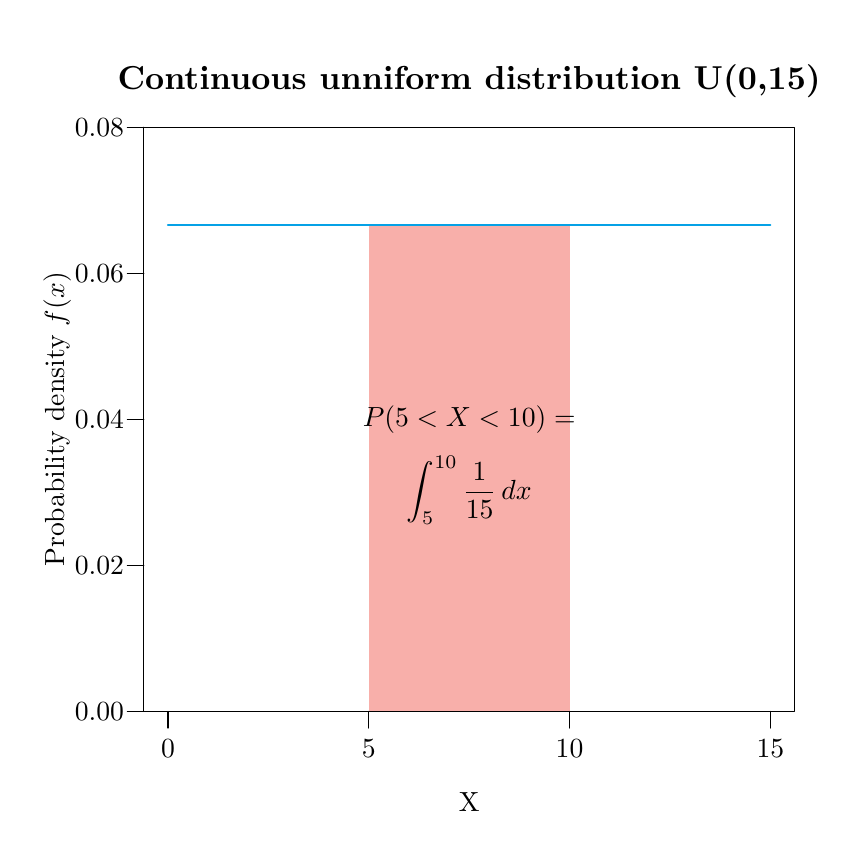
\begin{tikzpicture}[x=1pt,y=1pt]
\definecolor{fillColor}{RGB}{255,255,255}
\path[use as bounding box,fill=fillColor,fill opacity=0.00] (0,0) rectangle (289.08,289.08);
\begin{scope}
\path[clip] (  0.00,  0.00) rectangle (289.08,289.08);
\definecolor{drawColor}{RGB}{0,0,0}

\path[draw=drawColor,line width= 0.4pt,line join=round,line cap=round] ( 50.71, 42.00) -- (268.37, 42.00);

\path[draw=drawColor,line width= 0.4pt,line join=round,line cap=round] ( 50.71, 42.00) -- ( 50.71, 36.00);

\path[draw=drawColor,line width= 0.4pt,line join=round,line cap=round] (123.26, 42.00) -- (123.26, 36.00);

\path[draw=drawColor,line width= 0.4pt,line join=round,line cap=round] (195.82, 42.00) -- (195.82, 36.00);

\path[draw=drawColor,line width= 0.4pt,line join=round,line cap=round] (268.37, 42.00) -- (268.37, 36.00);

\node[text=drawColor,anchor=base,inner sep=0pt, outer sep=0pt, scale=  1.00] at ( 50.71, 25.20) {0};

\node[text=drawColor,anchor=base,inner sep=0pt, outer sep=0pt, scale=  1.00] at (123.26, 25.20) {5};

\node[text=drawColor,anchor=base,inner sep=0pt, outer sep=0pt, scale=  1.00] at (195.82, 25.20) {10};

\node[text=drawColor,anchor=base,inner sep=0pt, outer sep=0pt, scale=  1.00] at (268.37, 25.20) {15};

\path[draw=drawColor,line width= 0.4pt,line join=round,line cap=round] ( 42.00, 42.00) -- ( 42.00,253.08);

\path[draw=drawColor,line width= 0.4pt,line join=round,line cap=round] ( 42.00, 42.00) -- ( 36.00, 42.00);

\path[draw=drawColor,line width= 0.4pt,line join=round,line cap=round] ( 42.00, 94.77) -- ( 36.00, 94.77);

\path[draw=drawColor,line width= 0.4pt,line join=round,line cap=round] ( 42.00,147.54) -- ( 36.00,147.54);

\path[draw=drawColor,line width= 0.4pt,line join=round,line cap=round] ( 42.00,200.31) -- ( 36.00,200.31);

\path[draw=drawColor,line width= 0.4pt,line join=round,line cap=round] ( 42.00,253.08) -- ( 36.00,253.08);

\node[text=drawColor,anchor=base east,inner sep=0pt, outer sep=0pt, scale=  1.00] at ( 34.80, 38.56) {0.00};

\node[text=drawColor,anchor=base east,inner sep=0pt, outer sep=0pt, scale=  1.00] at ( 34.80, 91.33) {0.02};

\node[text=drawColor,anchor=base east,inner sep=0pt, outer sep=0pt, scale=  1.00] at ( 34.80,144.10) {0.04};

\node[text=drawColor,anchor=base east,inner sep=0pt, outer sep=0pt, scale=  1.00] at ( 34.80,196.87) {0.06};

\node[text=drawColor,anchor=base east,inner sep=0pt, outer sep=0pt, scale=  1.00] at ( 34.80,249.64) {0.08};

\path[draw=drawColor,line width= 0.4pt,line join=round,line cap=round] ( 42.00, 42.00) --
	(277.08, 42.00) --
	(277.08,253.08) --
	( 42.00,253.08) --
	( 42.00, 42.00);
\end{scope}
\begin{scope}
\path[clip] (  0.00,  0.00) rectangle (289.08,289.08);
\definecolor{drawColor}{RGB}{0,0,0}

\node[text=drawColor,anchor=base,inner sep=0pt, outer sep=0pt, scale=  1.20] at (159.54,266.89) {\bfseries Continuous unniform distribution U(0,15)};

\node[text=drawColor,anchor=base,inner sep=0pt, outer sep=0pt, scale=  1.00] at (159.54,  6.00) {X};

\node[text=drawColor,rotate= 90.00,anchor=base,inner sep=0pt, outer sep=0pt, scale=  1.00] at ( 13.20,147.54) {Probability density $f(x)$};
\end{scope}
\begin{scope}
\path[clip] ( 42.00, 42.00) rectangle (277.08,253.08);
\definecolor{fillColor}{RGB}{238,50,36}

\path[fill=fillColor,fill opacity=0.39] (123.26, 42.00) --
	(123.26,217.90) --
	(195.82,217.90) --
	(195.82, 42.00) --
	cycle;
\definecolor{drawColor}{RGB}{5,161,230}

\path[draw=drawColor,line width= 0.8pt,line join=round,line cap=round] ( 50.71,217.90) --
	(123.26,217.90) --
	(195.82,217.90) --
	(268.37,217.90);
\definecolor{drawColor}{RGB}{0,0,0}

\node[text=drawColor,anchor=base,inner sep=0pt, outer sep=0pt, scale=  1.00] at (159.54,145.04) {$P(5<X<10)=$};

\node[text=drawColor,anchor=base,inner sep=0pt, outer sep=0pt, scale=  1.00] at (159.54,118.65) {$\displaystyle \int_5^{10} \frac{1}{15}\,dx$};
\end{scope}
\end{tikzpicture}
}}
\end{center}
\end{column}
\end{columns}
Además, el tiempo medio de espera será $\mu=\frac{0+15}{2}=7.5$ minutos.

\end{frame}
% 
% 
% \subsection{Distribución Normal}
% 
% %---------------------------------------------------------------------slide----
% \begin{frame}
% \frametitle{Distribución Normal $N(\mu,\sigma)$}
% El modelo de distribución normal es, sin duda, el modelo de distribución continuo más importante, ya que es el que más a menudo se presenta
% en la naturaleza.
% \begin{definition}[Distribución Normal]
% Una variable aleatoria continua $X$ sigue un modelo de distribución \emph{normal} $N(\mu,\sigma)$ si su recorrido es $\mathbb{R}$ y su función de densidad vale
% \[
% f(x)= \frac{1}{\sigma\sqrt{2\pi}}e^{-\frac{(x-\mu)^2}{2\sigma^2}}.
% \]
% \end{definition}
% 
% La distribución normal depende de dos parámetros $\mu$ y $\sigma$ que son, precisamente, su media y desviación típica.
% 
% \note{
% El modelo de distribución normal es, sin duda, el modelo de distribución continuo más importante, ya que es el que más a menudo se presenta
% en la naturaleza, sobre todo en variables continuas biológicas.
% 
% \begin{definition}[Distribución Normal]
% Una variable aleatoria continua $X$ sigue un modelo de distribución \emph{normal} $N(\mu,\sigma)$ si su recorrido es $\mathbb{R}$ y su función de densidad vale
% \[
% f(x)= \frac{1}{\sigma\sqrt{2\pi}}e^{-\frac{(x-\mu)^2}{2\sigma^2}}.
% \]
% \end{definition}
% 
% La distribución normal depende de dos parámetros $\mu$ y $\sigma$ que son, precisamente, su media y desviación típica.
% }
% \end{frame}
% 
% 
% %---------------------------------------------------------------------slide----
% \begin{frame}
% \frametitle{Función de densidad de la Normal $N(\mu,\sigma)$}
% La gráfica de la función de densidad de la distribución normal tiene forma de una especie de campana, conocida como \emph{campana de Gauss}
% (en honor a su descubridor), y está centrada en la media $\mu$.
% \begin{center}
% \scalebox{0.65}{\input{img/variables_aleatorias_continuas/funcion_densidad_normal}}
% \end{center}
% 
% \note{
% La gráfica de la función de densidad de la distribución normal tiene forma de una especie de campana, conocida como \emph{campana de Gauss}
% (en honor a su descubridor), y está centrada en la media $\mu$.
% }
% \end{frame}
% 
% 
% %---------------------------------------------------------------------slide----
% \begin{frame}
% \frametitle{Función de densidad de la Normal $N(\mu,\sigma)$}
% La forma de la campana de Gauss depende de sus dos parámetros:
% \begin{itemize}
% \item La media $\mu$ determina dónde está centrada.
% \item La desviación típica $\sigma$ determina su anchura.
% \end{itemize} 
% \begin{center}
% \scalebox{0.5}{\input{img/variables_aleatorias_continuas/funcion_densidad_normales_distinta_media}}
% \quad
% \scalebox{0.5}{\input{img/variables_aleatorias_continuas/funcion_densidad_normales_distinta_varianza}}
% \end{center}
% 
% \note{
% La forma de la campana de Gauss depende de sus dos parámetros:
% \begin{itemize}
% \item Por un lado, ya hemos visto que la media $\mu$ determina dónde está centrada. En la gráfica de la izquierda podemos ver las funciones
% de densidad de dos normales, una con media 0 y desviación típica 1, y otra con media 2 y desviación típica 1. Como se ve, ambas gráficas son
% idénticas, salvo que la primera está centrada en el 0 y la segunda en el 2.
% \item Por otro lado, la desviación típica $\sigma$, al ser una medida de la dispersión de la población, determina su anchura. En la gráfica
% de la derecha podemos ver las funciones de densidad de dos normales con la misma media 0, y desviaciones típicas 1, y 2 respectivamente.
% Como se ve, ambas están centradas en el 0, pero la primera es más estrecha que la segunda al tener menos dispersión. 
% \end{itemize} 
% }
% \end{frame}
% 
% 
% %---------------------------------------------------------------------slide----
% \begin{frame}
% \frametitle{Función de distribución de la Normal $N(\mu,\sigma)$}
% Por su parte, la gráfica de la función de distribución tiene forma de S. 
% \begin{center}
% \scalebox{0.7}{\input{img/variables_aleatorias_continuas/funcion_distribucion_normal}}
% \end{center}
% 
% \note{
% Por su parte, la gráfica de la función de distribución de una normal siempre tiene forma de S. 
% }
% \end{frame}
% 
% 
% %---------------------------------------------------------------------slide----
% \begin{frame}
% \frametitle{Propiedades de la distribución Normal}
% \begin{itemize}
% \item La función de densidad es simétrica respecto a la media y por tanto, su coeficiente de asimetría es $g_1=0$.
% \item También es mesocúrtica, y por tanto, su coeficiente de apuntamiento vale $g_2=0$.
% \item La media, la mediana y la moda coinciden
% \[
% \mu = Me = Mo.
% \]
% \item Tiende asintóticamente a 0 cuando $x$ tiende a $\pm \infty$.
% \end{itemize}
% 
% \note{
% La distribución normal tiene propiedades muy interesantes:
% \begin{itemize}
% \item La función de densidad es simétrica respecto a la media y por tanto, su coeficiente de asimetría es $g_1=0$.
% \item También es mesocúrtica, y por tanto, su coeficiente de apuntamiento vale $g_2=0$. Recordemos que el apuntamiento de cualquier variable
% se compara precisamente con el apuntamiento de la distribución normal, ya que al ser esta la distribución más común, se toma como
% referencia.
% \item De nuevo, al ser simétrica con respecto a la media, hasta la media tendremos acumulada la mitad de la probabilidad, y por tanto la
% media coincide con la mediana, y también con la moda, ya que sobre la media se alcanza el máximo de la función de densidad.
% \[
% \mu = Me = Mo.
% \]
% \item Tiende asintóticamente a 0 cuando $x$ tiende a $\pm \infty$.
% \end{itemize}
% }
% \end{frame}
% 
% 
% %---------------------------------------------------------------------slide----
% \begin{frame}
% \frametitle{Propiedades de la distribución Normal}
% \begin{itemize}
% \item Se cumple que
% \begin{align*}
% & P(\mu-\sigma \leq X \leq \mu+\sigma) = 0.68,\\
% & P(\mu-2\sigma \leq X \leq \mu+2\sigma) = 0.95,\\
% & P(\mu-3\sigma \leq X \leq \mu+3\sigma) = 0.99.
% \end{align*}
% \end{itemize}
% \begin{center}
% \scalebox{0.6}{\input{img/variables_aleatorias_continuas/propiedades_normal}}
% \end{center}
% 
% \note{
% Y también se cumple que
% \begin{align*}
% & P(\mu-\sigma \leq X \leq \mu+\sigma) = 0.68,\\
% & P(\mu-2\sigma \leq X \leq \mu+2\sigma) = 0.95,\\
% & P(\mu-3\sigma \leq X \leq \mu+3\sigma) = 0.99.
% \end{align*}
% }
% es decir, casi la totalidad de los individuos de la población presentarán valores entre la media menos tres veces la desviación típica, y la
% media mas tres veces la desviación típica.
% \end{frame}
% 
% 
% %---------------------------------------------------------------------slide----
% \begin{frame}
% \frametitle{Propiedades de la distribución Normal}
% \framesubtitle{Ejemplo}
% En un estudio se ha comprobado que el nivel de colesterol total en mujeres
% sanas de entre 40 y 50 años sigue una distribución normal de media de 210 mg/dl y desviación
% típica 20 mg/dl. 
% \emph{¿Qué quiere decir esto?}
% 
% Atendiendo a las propiedades de la campana de Gauss, se tiene que 
% \begin{itemize}
% \item El 68\% de las mujeres sanas tendrán el colesterol entre $210\pm 20$ mg/dl, es decir, entre 190 y 230 mg/dl.
% \item El 95\% de las mujeres sanas tendrán el colesterol entre $210\pm 2\cdot 20$ mg/dl, es decir, entre 170 y 250
% mg/dl.
% \item El 99\% de las mujeres sanas tendrán el colesterol entre $210\pm 3\cdot 20$ mg/dl, es decir, entre 150 y 270
% mg/dl.
% \end{itemize}
% 
% En la analítica sanguínea suele utilizarse el intervalo $\mu\pm 2\sigma$ para detectar posibles patologías. En el caso
% del coresterol, dicho intervalo es $[170\text{ mg/dl}, 250\text{ mg/dl}]$. Cuando una persona tiene el colesterol fuera
% de estos límites, se tiende a pensar que tiene alguna patología, aunque ciertamente podría estar sana, pero la
% probabilidad de que eso ocurra es sólo de un 5\%.
% 
% \note{
% Veamos una aplicación de estas propiedades. 
% 
% En un estudio se ha comprobado que el nivel de colesterol total en mujeres sanas de entre 40 y 50 años sigue una distribución normal de
% media de 210 mg/dl y desviación típica 20 mg/dl. 
% \emph{¿Qué quiere decir esto?}
% 
% Atendiendo a las propiedades de la campana de Gauss, se tiene que 
% \begin{itemize}
% \item El 68\% de las mujeres sanas tendrán el colesterol entre $210\pm 20$ mg/dl, es decir, entre 190 y 230 mg/dl.
% \item El 95\% de las mujeres sanas tendrán el colesterol entre $210\pm 2\cdot 20$ mg/dl, es decir, entre 170 y 250
% mg/dl.
% \item El 99\% de las mujeres sanas tendrán el colesterol entre $210\pm 3\cdot 20$ mg/dl, es decir, entre 150 y 270
% mg/dl.
% \end{itemize}
% 
% En la analítica sanguínea suele utilizarse el intervalo $\mu\pm 2\sigma$ para detectar posibles patologías. En el caso
% del coresterol, dicho intervalo es $[170\text{ mg/dl}, 250\text{ mg/dl}]$. Cuando una persona tiene el colesterol fuera
% de estos límites, se tiende a pensar que tiene alguna patología, aunque ciertamente podría estar sana, pero la
% probabilidad de que eso ocurra es sólo de un 5\%.
% }
% \end{frame}
% 
% 
% %---------------------------------------------------------------------slide----
% \begin{frame}
% \frametitle{El teorema central del límite}
% El comportamiento anterior lo presentan muchas variables continuas físicas y biológicas.
% 
% Si se piensa por ejemplo en la distribución de las estaturas, se verá que la mayor parte de los individuos presentan estaturas en torno a la
% media, tanto por arriba, como por debajo, pero que a medida que van alejándose de la media, cada vez hay menos individuos con dichas
% estaturas.
% 
% La justificación de que la distribución normal aparezca de manera tan frecuente en la naturaleza la encontramos en el
% \structure{\textbf{teorema central del límite}}, que veremos más adelante, y que establece que si una variable aleatoria $X$ proviene de un
% experimento aleatorio cuyos resultados son debidos a un conjunto muy grande de causas independientes que actúan sumando sus efectos,
% entonces $X$ sigue una distribución aproximadamente normal.
% 
% \note{
% Se ha observado que la mayor parte de las variables continuas físicas y biológicas presentan una distribucón con forma de campana de Gauss.
% 
% Si se piensa por ejemplo en la distribución de las estaturas, se verá que la mayor parte de los individuos presentan estaturas en torno a la
% media, tanto por arriba, como por debajo, pero que a medida que van alejándose de la media, cada vez hay menos individuos con dichas
% estaturas.
% 
% La justificación de que la distribución normal aparezca de manera tan frecuente en la naturaleza la encontramos en el
% \structure{\textbf{teorema central del límite}}, que veremos más detenidamente en el siguiente tema, y que establece que si una variable
% aleatoria $X$ proviene de un experimento aleatorio cuyos resultados son debidos a un conjunto muy grande de causas independientes que actúan
% sumando sus efectos, entonces $X$ sigue una distribución aproximadamente normal.
% 
% Si pensamos en cualquier variable biológica, como por ejemplo la tensión arterial, rápidamente podremos identificar multitud de factores que
% influyen en ella, como por ejemplo la edad, el sexo, la dieta, el ejercicio físico, si se fuma o no, etc. El valor de la tensión arterial en
% un individuo es el resultado de todos estos factores que suman sus efectos de manera independiente, y por ello, el el colesterol acaba
% teniendo una distribución normal.
% }
% \end{frame}
% 
% 
% %---------------------------------------------------------------------slide----
% \begin{frame}
% \frametitle{La distribución Normal estándar $N(0,1)$}
% De todas las distribuciones normales, la más importante es la que tiene media $\mu=0$ y desviación típica $\sigma=1$,
% que se conoce como \structure{\textbf{normal estándar}} y se designa por $Z$.
% \begin{center}
% \scalebox{0.65}{\input{img/variables_aleatorias_continuas/funcion_densidad_normal_estandar}}
% \end{center}
% 
% \note{
% De todas las distribuciones normales, la más importante es la que tiene media $\mu=0$ y desviación típica $\sigma=1$,
% que se conoce como \structure{\textbf{normal estándar}} y se designa por $Z$.
% 
% Su función de densidad será una campana de Gauss centrada en el 0, en la que el 99\% de los individuos estarán entre -3 y 3. 
% }
% \end{frame}
% 
% 
% %---------------------------------------------------------------------slide----
% \begin{frame}
% \frametitle{Cálculo de probabilidades con la Normal estándar}
% \framesubtitle{Manejo de la tabla de la función de distribución}
% Para evitar tener que calcular probabilidades integrando la función de densidad de la normal estándar se suele utilizar su función de
% distribución.
% 
% Habitualmente se suele manejar una tabla con los valores de la función de distribución tabulados cada centésima. 
% \begin{columns}
% \begin{column}{0.47\textwidth}
% \begin{center}
% Ejemplo $P(Z\leq 0.52)$
% 
% \scalebox{0.8}{\input{img/variables_aleatorias_continuas/tabla_normal}}
% 
% $0.52 \rightarrow $ fila $0.5$ + columna $0.02$
% \end{center}
% \end{column}
% \begin{column}{0.53\textwidth}
% \scalebox{0.6}{\input{img/variables_aleatorias_continuas/calculo_probabilidades_normal_estandar}}
% \end{column}
% \end{columns}
% 
% \note{
% Para evitar tener que calcular probabilidades integrando la función de densidad de la normal estándar se suele utilizar su función de
% distribución.
% 
% Habitualmente se suele manejar una tabla con los valores de la función de distribución tabulados cada centésima. En esta tabla, la primera
% columna contiene las décimas y la primera fila las centésimas, de forma que si por ejemplo queremos medir la probabilidad acumulada hasta el
% $0.52$, tenemos que ir hasta la casilla correspondiente a la fila $0.5$  (5 décimas) y hasta la columna $0.02$ (2 centésimas), donde aparece
% la probabilidad acumulada $0.6985$ y esta sería el área que queda por debajo de la campana de Gauss de la normal estándar entre $-\infty$ y
% $0.52$.
% }
% \end{frame}
% 
% 
% %---------------------------------------------------------------------slide----
% \begin{frame}
% \frametitle{Cálculo de probabilidades con la Normal estándar}
% \framesubtitle{Probabilidades acumuladas por encima de un valor}
% Cuando tengamos que calcular probabilidades acumuladas por encima de un determinado valor, podemos hacerlo por medio de la probabilidad del
% suceso contrario.
% 
% Por ejemplo
% \[
% P(Z>0.52) =1-P(Z\leq 0.52) = 1-F(0.52) = 1 - 0.6985 = 0.3015.
% \]
% \begin{center}
% \scalebox{0.55}{\input{img/variables_aleatorias_continuas/calculo_probabilidades_derecha_normal_estandar}}
% \end{center}
% 
% \note{
% Cuando tengamos que calcular probabilidades acumuladas por encima de un determinado valor, podemos hacerlo por medio de la probabilidad del
% suceso contrario, ya que la función de distribución siempre mide probabilidades acumuladas por debajo de cada valor. 
% 
% Así, la probabilidad acumulada por encima de $0.52$, será 1 menos la probabilidad acumulada por debajo de dicho valor, que como hemos visto
% en la tabla, valía $0.6985$, lo que nos da $0.3015$. Esto es lógico, ya que si el área total por debajo de la campana de Gauss es 1, el área
% acumulada por encima de $0.52$ será 1 menos el área que quede por debajo de este valor. 
% }
% \end{frame}
% 
% 
% %---------------------------------------------------------------------slide----
% \begin{frame}
% \frametitle{Tipificación}
% Ya se ha visto cómo calcular probabilidades con una distribución normal estándar, pero \emph{¿qué hacer cuando la
% distribución normal no es la estándar?}
% 
% Afortunadamente, siempre se puede transformar una variable normal para convertirla en una normal estándar. 
% \begin{teorema}[Tipificación]
% Si $X$ es una variable normal de media $\mu$ y desviación típica $\sigma$, entonces la variable resultante de restarle a $X$ su media y
% dividir por su desviación típica, sigue un modelo de distribución normal estándar:
% \[
% X\sim N(\mu,\sigma) \Rightarrow Z=\frac{X-\mu}{\sigma}\sim N(0,1).
% \]
% Esta transformación lineal se conoce como \emph{transformación de tipificación} y la variable resultante $Z$ se conoce como \emph{normal
% tipificada}.
% \end{teorema} 
% 
% Así pues, para calcular probabilidades de una variable normal que no sea la normal estándar, se aplica primero la transformación de
% tipificación y después se puede utilizar la función de distribución de la normal estándar.
% 
% \note{
% Ya se ha visto cómo calcular probabilidades con una distribución normal estándar, pero \emph{¿qué hacer cuando la
% distribución normal no es la estándar?}
% 
% Afortunadamente, siempre se puede transformar una variable normal para convertirla en una normal estándar tipificándola.
% \begin{teorema}[Tipificación]
% Si $X$ es una variable normal de media $\mu$ y desviación típica $\sigma$, entonces la variable resultante de restarle a $X$ su media y
% dividir por su desviación típica, sigue un modelo de distribución normal estándar:
% \[
% X\sim N(\mu,\sigma) \Rightarrow Z=\frac{X-\mu}{\sigma}\sim N(0,1).
% \]
% Esta transformación lineal se conoce como \emph{transformación de tipificación} y la variable resultante $Z$ se conoce como \emph{normal
% tipificada}.
% \end{teorema} 
% 
% Así pues, para calcular probabilidades de una variable normal que no sea la normal estándar, tendremos que aplicar la transformación de
% tipificación primero y después se puede utilizar la tabla de la función de distribución de la normal estándar.
% }
% \end{frame}
% 
% 
% %---------------------------------------------------------------------slide----
% \begin{frame}
% \frametitle{Cálculo de probabilidades tipificando}
% \framesubtitle{Ejemplo}
% Supóngase que la nota de un examen sigue un modelo de distribución de probabilidad normal $N(\mu=6,\sigma=1.5)$. \emph{¿Qué porcentaje de
% suspensos habrá en la población?}
% 
% Para responder a esta pregunta necesitamos calcular la probabilidad $P(X<5)$. Como $X$ no es la normal estándar, se le aplica la
% transformación de tipificación $Z=\displaymath \frac{X-\mu}{\sigma} = \frac{X-6}{1.5}$:
% \[
% P(X<5) = P\left(\frac{X-6}{1.5}<\frac{5-6}{1.5}\right) = P(Z<-0.67).
% \]
% Después se mira en la tabla de la función de distribución de la normal estándar:
% \[
% P(Z<-0.67) = F(-0.67) = 0.2514.
% \]
% 
% Así pues, habrán suspendido el $25.14\%$ de los alumnos. 
% 
% \note{
% Veamos un ejemplo. 
% 
% Supóngase que la nota de un examen sigue un modelo de distribución de probabilidad normal $N(\mu=6,\sigma=1.5)$. \emph{¿Qué porcentaje de
% suspensos habrá en la población?}
% 
% Para responder a esta pregunta necesitamos calcular la probabilidad de que la nota sea inferior a 5. Como $X$ no es la normal estándar, se
% le aplica la transformación de tipificación, que es $Z=\displaymath \frac{X-\mu}{\sigma} = \frac{X-6}{1.5}$. Por tanto, 
% \[
% P(X<5) = P\left(\frac{X-6}{1.5}<\frac{5-6}{1.5}\right) = P(Z<-0.67).
% \]
% Después sólo queda mirar en tabla de la función de distribución de la normal estándar y observar que la probabilidad acumulada hasta el
% $-0.67$ es $0.2514$.
% 
% Así pues, habrán suspendido el $25.14\%$ de los alumnos. 
% }
% \end{frame}
% 
% 
% \subsection{Distribución Chi-cuadrado}
% 
% %---------------------------------------------------------------------slide----
% \begin{frame}
% \frametitle{Distribución chi-cuadrado $\chi^2(n)$}
% \begin{definition}[Distribución chi-cuadrado $\chi^2(n)$]
% Si  $Z_1,\ldots,Z_n$ son $n$ variables aleatorias normales estándar independientes, entonces la suma de sus cuadrados sigue un modelo de
% distribución \emph{chi-cuadrado de $n$ grados de libertad}:
% \[
% \chi^2(n) = Z_1^2+\cdots +Z_n^2.
% \]
% \end{definition}
% Su recorrido es  $\mathbb{R}^+$ y su media y varianza valen
% \[
% \mu = n, \qquad \sigma^2 = 2n.
% \]
% Como se verá más adelante, la distribución chi-cuadrado juega un papel importante en la estimación de la varianza poblacional y en el
% estudio de la relación entre variables cualitativas.
% 
% \note{
% Las distribuciones que veremos a continuación son distribuciones que siguen algunos de los estadísticos observados en las muestras
% aleatorias. Su principal utilidad se verá en el siguiente tema.
% 
% El primer modelo de distribución es el modelo chi-cuadrado.
% 
% Si  $Z_1,\ldots,Z_n$ son $n$ variables aleatorias normales estándar independientes, entonces
% la suma de sus cuadrados sigue un modelo de distribución \emph{chi-cuadrado de $n$ grados de libertad}:
% \[
% \chi^2(n) = Z_1^2+\cdots +Z_n^2.
% \]
% 
% Se cumple que su recorrido es  $\mathbb{R}^+$, su media vale $\mu=n$ y su varianza vale $\sigma^2 = 2n$.
% 
% Como se verá más adelante, la distribución chi-cuadrado juega un papel importante en la estimación de la varianza poblacional y en el
% estudio de la relación entre variables cualitativas.
% }
% \end{frame}
% 
% 
% %---------------------------------------------------------------------slide----
% \begin{frame}
% \frametitle{Función de densidad de la distribución chi-cuadrado}
% 
% \begin{center}
% \scalebox{0.8}{\input{img/variables_aleatorias_continuas/funcion_densidad_chi_cuadrado}}
% \end{center}
% 
% \note{
% Aquí tenemos las gráfica de la función de densidad de varias distribuciones chi-cuadrado con distintos grados de libertad. Como se puede
% apreciar, esta distribución, por ser la suma de cuadrados, no presenta valores negativos, y a diferencia de la normal, siempre es asimétrica
% hacia la izquierda.
% }
% \end{frame}
% 
% 
% %---------------------------------------------------------------------slide----
% \begin{frame}
% \frametitle{Propiedades de la distribución chi-cuadrado $\chi^2(n)$}
% \begin{itemize}
% \item No toma valores negativos.
% \item Si $X\sim \chi^2(n)$ e $Y\sim \chi^2(m)$, entonces
% \[
% X+Y \sim \chi^2(n+m).
% \]
% \item Al aumentar el número de grados de libertad, se aproxima asintóticamente a una normal.
% \end{itemize}
% 
% \note{
% Algunas propiedades que tiene la distribución chi-cuadrado son:
% \begin{itemize}
% \item No toma valores negativos.
% \item Si $X\sim \chi^2(n)$ e $Y\sim \chi^2(m)$, entonces
% \[
% X+Y \sim \chi^2(n+m).
% \]
% \item Al aumentar el número de grados de libertad, se aproxima asintóticamente a una normal.
% \end{itemize}
% }
% \end{frame}
% 
% 
% \subsection{Distribución T de Student}
% 
% %---------------------------------------------------------------------slide----
% \begin{frame}
% \frametitle{Distribución T de Student $T(n)$}
% \begin{definition}[Distribución T de Student $T(n)$]
% Si  $Z\sim N(0,1)$ es una variable aleatoria normal estándar y $X\sim \chi^2(n)$ es una variable aleatoria chi-cuadrado de $n$ grados de
% libertad, ambas independientes, entonces la variable
% \[
% T = \frac{Z}{\sqrt{X/n}},
% \]
% sigue un modelo de distribución \emph{T de Student de $n$ grados de libertad}.
% \end{definition}
% 
% Su recorrido es $\mathbb{R}$ y su media y varianza valen
% \[
% \mu = 0, \qquad \sigma^2 = \frac{n}{n-2} \mbox{ si $n>2$}.
% \]
% 
% Como se verá más adelante, la distribución T de Student juega un papel importante en la estimación la media poblacional.
% 
% \note{
% \begin{definition}[Distribución T de Student $T(n)$]
% Si  $Z\sim N(0,1)$ es una variable aleatoria normal estándar y $X\sim \chi^2(n)$ es una variable aleatoria chi-cuadrado de $n$ grados de
% libertad, ambas independientes, entonces la variable
% \[
% T = \frac{Z}{\sqrt{X/n}},
% \]
% sigue un modelo de distribución \emph{T de Student de $n$ grados de libertad}.
% \end{definition}
% 
% Se cumple que su recorrido es $\mathbb{R}$ y su media vale $\mu=0$ y su varianza vale
% \[
% \sigma^2 = \frac{n}{n-2} \mbox{ si $n>2$}.
% \]
% 
% Como se verá más adelante, la distribución T de Student juega un papel importante en la estimación la media poblacional.
% }
% \end{frame}
% 
% 
% %---------------------------------------------------------------------slide----
% \begin{frame}
% \frametitle{Función de densidad de la distribución T de Student}
% 
% \begin{center}
% \scalebox{0.8}{\input{img/variables_aleatorias_continuas/funcion_densidad_t_student}}
% \end{center}
% 
% \note{
% Aquí tenemos las gráfica de la función de densidad de varias distribuciones T de student con distintos grados de libertad. Como se puede
% apreciar, esta distribución está centrada en el 0 y es muy parecida a la normal estándar, aunque un poco más platicúrtica. 
% }
% \end{frame}
% 
% 
% %---------------------------------------------------------------------slide----
% \begin{frame}
% \frametitle{Propiedades de la distribución T de Student $T(n)$}
% \begin{itemize}
% \item Es simétrica con respecto a su media $\mu=0$.
% \item Es muy similar a la normal estándar, pero algo más platicúrtica. Además, a medida que aumentan los grados de libertad, la gráfica de la distribución tiende hacia la de la normal estándar, hasta llegar a ser prácticamente iguales para $n\geq 30$.
% \[
% T(n)\stackrel{n\rightarrow \infty}{\approx}N(0,1).
% \]
% \end{itemize}
% 
% \note{
% Algunas propiedades que tiene la distribución T de student son:
% \begin{itemize}
% \item Es simétrica con respecto a su media $\mu=0$.
% \item Como ya hemos dicho, es muy similar a la normal estándar, pero algo más platicúrtica. Además, a medida que aumentan los grados de
% libertad, la gráfica de la distribución tiende hacia la de la normal estándar, hasta llegar a ser prácticamente iguales para $n\geq 30$.
% \[
% T(n)\stackrel{n\rightarrow \infty}{\approx}N(0,1).
% \]
% \end{itemize}
% }
% \end{frame}
% 
% 
% \subsection{Distribución F de Fisher-Snedecor}
% 
% %---------------------------------------------------------------------slide----
% \begin{frame}
% \frametitle{Distribución F de Fisher-Snedecor $F(m,n)$}
% \begin{definition}[Distribución F de Fisher-Snedecor $F(m,n)$]
% Si  $X\sim \chi^2(m)$ es una variable aleatoria chi-cuadrado de $m$ grados de libertad e $Y\sim \chi^2(n)$ es otra variable aleatoria
% chi-cuadrado de $n$ grados de libertad, ambas independientes, entonces la variable
% \[
% F = \frac{X/m}{Y/n},
% \]
% sigue un modelo de distribución \emph{F de Fisher-Snedecor de $m$ y $n$ grados de libertad}.
% \end{definition}
% 
% Su recorrido es $\mathbb{R}^+$ y su media y varianza valen
% \[
% \mu = \frac{n}{n-2}, \qquad \sigma^2 =\frac{2n^2(m+n−2)}{m(n-2)^2(n-4)}\mbox{ si $n>4$}.
% \]
% 
% Como se verá más adelante, la distribución F de Fisher-Snedecor juega un papel importante en la comparación de varianzas poblacionales y en
% el análisis de la varianza.
% 
% \note{
% \begin{definition}[Distribución F de Fisher-Snedecor $F(m,n)$]
% Si  $X\sim \chi^2(m)$ es una variable aleatoria chi-cuadrado de $m$ grados de libertad e $Y\sim \chi^2(n)$ es otra variable aleatoria
% chi-cuadrado de $n$ grados de libertad, ambas independientes, entonces la variable
% \[
% F = \frac{X/m}{Y/n},
% \]
% sigue un modelo de distribución \emph{F de Fisher-Snedecor de $m$ y $n$ grados de libertad}.
% \end{definition}
% 
% Se cumple que su recorrido es $\mathbb{R}^+$ y su media vale
% \[
% \mu = \frac{n}{n-2},
% \]
% y su varianza 
% \[
% \sigma^2 =\frac{2n^2(m+n−2)}{m(n-2)^2(n-4)}\mbox{ si $n>4$}.
% \]
% 
% Como se verá más adelante, la distribución F de Fisher-Snedecor juega un papel importante en la comparación de varianzas poblacionales y en
% el análisis de la varianza.
% }
% \end{frame}
% 
% 
% %---------------------------------------------------------------------slide----
% \begin{frame}
% \frametitle{Función de densidad de la distribución F de Fisher-Snedecor $F(m,n)$}
% 
% \begin{center}
% \scalebox{0.75}{\input{img/variables_aleatorias_continuas/funcion_densidad_f_fisher}}
% \end{center}
% 
% \note{
% Aquí tenemos las gráfica de la función de densidad de varias distribuciones F de Fisher con distintos grados de libertad. Como se puede
% apreciar, al igual que la distribución chi-cuadrado, no presenta valores negativos, y siempre es asimétrica hacia la izquierda.
% }
% \end{frame}
% 
% 
% %---------------------------------------------------------------------slide----
% \begin{frame}
% \frametitle{Propiedades de la distribución F de Fisher-Snedecor $F(m,n)$}
% \begin{itemize}
% \item No está definida para valores negativos.
% \item De la definición se deduce que
% \[
% F(m,n) =\frac{1}{F(n,m)}
% \]
% de manera que si llamamos $f(m,n)_p$ al valor que cumple que $P(F(m,n)≤f(m,n)_p)=p$, entonces se cumple
% \[                                          
% f(m,n)_p =\frac{1}{f(n,m)_{1−p}}
% \]
% Esto resulta muy útil para utilizar las tablas de su función de distribución.
% \end{itemize}
% 
% \note{
% Algunas propiedades que tiene la distribución F de Fisher son:
% \begin{itemize}
% \item No está definida para valores negativos.
% \item De la definición se deduce que
% \[
% F(m,n) =\frac{1}{F(n,m)}
% \]
% de manera que si llamamos $f(m,n)_p$ al valor que cumple que $P(F(m,n)≤f(m,n)_p)=p$, entonces se cumple
% \[                                          
% f(m,n)_p =\frac{1}{f(n,m)_{1−p}}
% \]
% Esto resulta muy útil para utilizar las tablas de su función de distribución.
% \end{itemize}
% }
% \end{frame}